

\pdfoutput=1

\documentclass[a4paper,USenglish]{lipics}

% \usepackage[utf8]{inputenc}

\usepackage[protrusion=true,expansion=true]{microtype}


\usepackage[style=numeric,
%  backref=true,
 isbn=false,
%  doi=false,
 maxnames=3,
 maxbibnames=99 ,                
 uniquename=init ,
]{biblatex}
\bibliography{literature.bib}

\usepackage{mdframed}
\usepackage{multicol}
\usepackage{ownstylelipics}

\usepackage{comment}
% \excludecomment{Long}\includecomment{Short}
\includecomment{Long}\excludecomment{Short}

% \pagestyle{plain}


\title{Terminal semantics for codata types in intensional Martin-L\"of type theory}

\author{Benedikt Ahrens}
\author{R\'egis Spadotti}

\affil{
Institut de Recherche en Informatique de Toulouse\\
Universit\'e Paul Sabatier, 
Toulouse}

\authorrunning{B.\ Ahrens and R.\ Spadotti}

\Copyright{Benedikt Ahrens and Régis Spadotti}
\subjclass{F.3.2 Semantics of Programming Languages}
% \subjclass{Dummy classification -- please refer to \url{http://www.acm.org/about/class/ccs98-html}}% mandatory: Please choose ACM 1998 classifications from http://www.acm.org/about/class/ccs98-html . E.g., cite as "F.1.1 Models of Computation". 
\keywords{relative comonad, Martin-Löf type theory, coinductive type, computer theorem proving}
% \keywords{Dummy keyword -- please provide 1--5 keywords}% mandatory: Please provide 1-5 keywords
% Author macros::end %%%%%%%%%%%%%%%%%%%%%%%%%%%%%%%%%%%%%%%%%%%%%%%%%

%Editor-only macros:: begin (do not touch as author)%%%%%%%%%%%%%%%%%%%%%%%%%%%%%%%%%%
\serieslogo{}%please provide filename (without suffix)
\volumeinfo%(easychair interface)
  {Billy Editor and Bill Editors}% editors
  {2}% number of editors: 1, 2, ....
  {Conference title on which this volume is based on}% event
  {1}% volume
  {1}% issue
  {1}% starting page number
\EventShortName{}
\DOI{10.4230/LIPIcs.xxx.yyy.p}% to be completed by the volume editor
% Editor-only macros::end %%%%%%%%%%%%%%%%%%%%%%%%%%%%%%%%%%%%%%%%%%%%%%%


\newcommand{\fat}[1]{\textbf{#1}}
\newcommand{\itemizedist}{.5em}

\begin{document}

\maketitle

% \tableofcontents

\begin{abstract}
 We study the notions of \emph{relative comonad} and \emph{comodule over a relative comonad}.
 We use these notions to give categorical semantics for the coinductive type families of streams and
 of infinite triangular matrices and their respective cosubstitution operations in intensional Martin-L\"of type theory.
 Our results are mechanized in the proof assistant \coq.
\end{abstract}




\section{Introduction}
 
 In this work, we study the notions of \emph{relative comonad} and \emph{comodule over a relative comonad}.
 We then use these notions for a case study in categorical semantics of coinductive data types in intensional Martin-Löf type theory (IMLTT): 
 we characterize two coinductive data types and their respective cosubstitution operations 
 in IMLTT via a universal property.
 The first codata type we consider is the \emph{homogeneous} type family of streams, parametrized by a base type.
 The second one is the \emph{heterogeneous} codata type family of infinite triangular matrices parametrized by the type of diagonal entries.
  In the rest of the introduction, we explain some of the vocabulary occurring in these first sentences:
  in \Cref{sec:mltt} we briefly introduce (intensional) Martin-Löf type theory. In \Cref{sec:sem_ind} we discuss inductive types and their semantics,
  before passing to \emph{co}inductive types in \Cref{sec:sem_coind}.
  We describe
  the difference between homogeneous and heterogeneous (co)data types in \Cref{sec:hom_het} and explain substitution for leaf-labeled trees and cosubstitution for node-labeled trees in \Cref{sec:cosubst}.
  The last sections of the introduction concern more \enquote{administrative} aspects of the present work.
  
  
 \subsection{Intensional Martin-Löf type theory}\label{sec:mltt}
 Martin-Löf type theory (MLTT) \parencite{martin_lof} is a dependent type theory developed in the 1970's, which provides a foundation of mathematics.
 It is based on the Curry-Howard isomorphism, that is, it treats logic as a fragment of the general type theory.
 There are two notions of \enquote{sameness} in Martin-Löf type theory, an external (judgmental) one, and an internal (propositional) one.
 The latter is internalized by  the \emph{Martin-Löf identity type}, which is an inductively defined binary relation on any given type.
 Its only constructor relates any term to itself, that is, the relation defined by the Martin-Löf identity type is the least reflexive relation on a given type.
 Judgmentally equal terms are always propositionally equal, but the converse is not always true.
 Indeed, one distinguishes two variants of type theory: in \emph{extensional} type theory, propositional equalities (i.e.\ terms of identity type)
 are reflected, via a \emph{reflection rule}, into the judgmental equality of the type theory.  
 Here, judgmental and propositional equality thus coincide.
 \emph{Intensional} Martin-L\"of type theory  lacks the reflection principle for the sake of decidability of type checking. 
 This variant forms the basis of the computer proof assistants \coq, \matita and \agda.

 
\begin{comment}
 \subsection{(Non-)wellfounded trees: (co)inductive types}
 
 A \emph{tree} is abstractly given by its \emph{root} and its \emph{subtrees}, which we think of as being attached to the root.
 Subtrees are themselves trees, again consisting of a root and attached subtrees.
 The roots of the various subtrees occurring in a tree are called \emph{nodes}. Among those, there are nodes without any subtrees, which are called \emph{leaves}.
 
%  TODO: fill in a picture of a tree
 
 
 

 A fundamental property of a tree is \emph{finiteness}. A tree is finite if it does not have a subtree of infinite length. 

 An inductive set/type specifies a set/type of trees of given shape, i.e.\ it specifies the set/type of nodes and, for each node, the number (cardinality) of subtrees 
 attached to that node. The trees defined inductively are \emph{finite} trees, i.e.\ no infinite chain of subtrees occurs in such a tree.
\end{comment}
 
\begin{Long}
 \subsection{Wellfounded trees and their semantics}\label{sec:sem_ind}
\end{Long}
\begin{Short}
 \paragraph*{Semantics of inductive types}
\end{Short}
 
 A tree is a special kind of graph (with labeled edges and unlabeled vertices), consisting of a \emph{root} (edge), 
 to which a number of \emph{subtrees} are attached. 
 The subtrees are themselves trees.
 The root of a tree and the roots of any subtrees are more generally called \emph{nodes}.
 We gather trees of a fixed shape into a set or type, depending on the foundations we work in. 
 The possible shapes of trees are given by two data:
 \begin{enumerate}
  \item the set/type of potential nodes and
  \item the number of subtrees attached to each node.
 \end{enumerate}
 Such a pair of data is called a \emph{signature}, and we are interested in the set/type of trees which are formed according to a given signature.
 
 A tree is called \emph{wellfounded} if any of its subtrees has finite length. In this section we consider the set/type of wellfounded trees of 
 a given signature. Such a set/type is called \emph{inductively generated} by the signature. Intuitively, this set/type is the least one stable under
 forming trees starting from leaves and attaching already constructed trees as subtrees to nodes.
 One might also consider \emph{potentially infinite}, i.e., non-wellfounded trees; these are called \emph{co}inductive and are the main object of this work.
 We discuss them in \Cref{sec:sem_coind}.
 
 
 Many objects in mathematics and logic can be represented as (wellfounded) \emph{trees}.
 For instance, a natural number can be considered as such a tree: let $\{S,Z\}$ be the set of possible nodes, 
 such that node $S$ always has one subtree and node $Z$ does not have any subtrees, i.e.\ $Z$ is a \emph{leaf}.
 The natural number $2$ is represented by the tree $S\longrightarrow S\longrightarrow Z$. 
 This example demonstrates the fundamental aspect of those tree-like objects: they can be used to model basic mathematical and logical objects.
 
  
 By \enquote{semantics of inductive types} we mean a mathematical description of the set/type of trees of a given signature. 
 More precisely, the purpose is to give a category-theoretic explanation to the above description as \enquote{the least set/type stable under forming trees}.
 However, the question of how to give such a characterization depends on the formal system we work in. 
 Below, we discuss briefly set-theoretic and type-theoretic such systems.
 
 In a set-theoretic setting, inductive sets are characterized as initial algebras for 
 some endofunctor on the category of sets \parencite{jacobs1997tutorial}.
 
 In a type-theoretic setting as given by Martin-L\"of type theory \parencite{martin_lof}, 
 two approaches to the semantics of inductive types have been studied: 
 one approach consists in showing that inductive types exist in a \emph{model} of the type theory,
 as is done, e.g., by \textcite{DBLP:journals/apal/MoerdijkP00}.
 Another approach is to prove that adding certain type-theoretic rules to the type theory---rules which postulate the existence
 of inductive types in the type theory---implies (or is equivalent to) the existence of a universal object \emph{within} type theory
 (see, e.g., \parencite{DBLP:conf/lics/AwodeyGS12, DBLP:journals/tcs/Dybjer97}).
 This latter approach is the one we adopt in the present work: we add axioms to intensional Martin-Löf type theory,
 postulating the existence of \emph{co}inductive types, see below.
 
 
%  When specifying a universal property within type theory, one needs a suitable notion of \emph{uniqueness} (of certain maps or morphisms).
%  The property of uniqueness (or more generally, equality) of morphisms may now be expressed in terms of either judgmental or propositional equality.
%   While in extensional type theory the two equalities coincide, in intensional type theory they do not, making this choice a crucial one.
%  
 
 The reflection rule equips \emph{extensional} type theory with extensional features similar to those of set theory.
 As a consequence, the characterization given by \textcite{DBLP:journals/tcs/Dybjer97} of an inductive type in extensional MLTT works as in set theory: 
 an inductive type constitutes the initial algebra for some endofunctor on the category of types.
 
 
  

 
  In \emph{intensional} Martin-Löf type theory the characterization of inductive types as initial algebras of some endofunctor fails 
  for a lack of function extensionality \parencite{DBLP:journals/tcs/Dybjer97}, 
  but it can be recovered \parencite{DBLP:conf/lics/AwodeyGS12} in an \emph{extension} of intensional MLTT called
  \emph{Homotopy Type Theory} \parencite{hottbook}.
  In this extension, function extensionality is provable from the \emph{Univalence Axiom}. 
 For a suitable definition of \emph{uniqueness}---\emph{contractibility} in HoTT jargon---one can prove uniqueness of the
 algebra morphisms out of the one whose carrier is given by the inductive type under consideration.
 The mentioned work \parencite{DBLP:conf/lics/AwodeyGS12} thus shows that the characterization of inductive types as initial algebras carries over 
 from extensional to intensional type theory if one adds an extensionality principle for functions and adapts the notion of uniqueness.
 
 
\begin{comment} 
%  TODO: put this at the beginning of cosubstitution
 The characterization of inductive sets/types as initial objects in some category
 has been extended to some \emph{heterogeneous}---also called \emph{nested}---inductive data types, e.g., the type of $\lambda$-terms,
 in different formulations \parencite{fpt, DBLP:journals/iandc/HirschowitzM10}.
 The main goal of these works is not just to characterize a data type via a universal property, but rather a data type
 \emph{equipped with a canonical, well-behaved substitution operation}.
\end{comment} 
 
\begin{Long}
 \subsection{Non-wellfounded trees: simply dualizing?}\label{sec:sem_coind}
\end{Long}
\begin{Short}
 \paragraph*{Coinductive types: simply dualizing?}
\end{Short}

  Coinductive sets/types describe sets/types of potentially \emph{infinite} trees, that is, trees that may have an infinite chain of subtrees---still formed according to some signature.
  An example of such a coinductive set/type is given by the \emph{co}natural numbers, which are specified by the same signature as the natural numbers.
  They consist of the elements of the natural numbers and an additional,
  infinite tree $S \longrightarrow S\longrightarrow S \longrightarrow \ldots$. 
  
 In a traditional set-theoretic setting, the theory of coinductive sets is completely dual to that of inductive sets:
  \emph{co}inductive sets are characterized as terminal coalgebras of 
 suitable endofunctors \parencite{jacobs1997tutorial}.
 
 In intensional Martin-Löf type theory, this duality between inductive and coinductive objects breaks. This is rooted in the 
 unsuitability of the Martin-Löf identity type to express sameness for inhabitants of coinductive types:
 while identity terms are inductively generated and hence necessarily finite, 
 a proof of sameness between coinductive terms---which represent infinite objects---constitutes a potentially infinite object itself.
 The type of such proofs hence cannot be exhaustively given by the (inductive) identity type.
 
 Instead of comparing two coinductive terms in Martin-Löf type theory up to identity, one defines a 
 binary coinductive relation called \emph{bisimilarity} on a given coinductive type, with respect to which one compares its inhabitants  \parencite{DBLP:conf/types/Coquand93}. 
 Categorically, \emph{bisimilarity} is given as the greatest---\emph{weakly terminal}---\emph{relation} on the coinductive type that is compatible with the coalgebra structure.
 
 Consequently, we consider two maps into a coinductive type to be the same if they are \emph{pointwise bisimilar}---an analogue
 to the aforementioned principle of function extensionality available in Homotopy Type Theory. 
 With these conventions, we give, in the present work, a characterization of some coinductive data types as \emph{terminal} object in some category 
 defined in intensional Martin-L\"of type theory.
 More precisely, we consider an example of \emph{homogeneous} codata type, streams, and 
 an example of \emph{heterogeneous} codata type, triangular matrices.
 For each of these examples we prove, 
 from type-theoretic rules specifying the respective codata type added to the basic rules of Martin-L\"of type theory,
 the existence of a terminal object in some category \emph{within IMLTT}.
 The objects of the considered categories are not plain coalgebras for some endofunctor, but rather coalgebras with extra structure.
 This extra structure accounts for a \emph{cosubstitution} operation with which the considered codata types are endowed in a canonical way.
 The cosubstitution operation is explained in \Cref{sec:cosubst}.

% \begin{Long}
%  We mention here work by \textcite{DBLP:conf/calco/Marchi05}, who studies the existence of coinductive types in models of \emph{extensional} Martin-L\"of type theory. In that work, no \emph{internal} characterization of coinductive types is given.
%  Furthermore, his work does not account for the mentioned cosubstitution operation.
% \end{Long}


\subsection{Homogeneous and heterogeneous trees}\label{sec:hom_het}

Instead of considering types of trees of a given signature, we consider, more generally, \emph{families} $T(X)$ of types of trees, families parametrized by a type $X$.
We call a tree $t:T(X)$ over $X$ \emph{homogeneous} if all of its subtrees are also trees over $X$, i.e.\, if all the subtrees are elements of $T(X)$.
A signature accordingly is called homogeneous if it only admits homogeneous trees.
On the other hand, a tree $t$ is called \emph{heterogeneous}, if its subtrees $t_i$ ($i : I$ for some indexing type $I$) are trees over 
type $F_i(X)$ for maps of types $F_i : \Set \to \Set$. Obviously, for $F_i$ the identity, we obtain homogeneous trees; heterogeneous trees are thus more general than
homogeneous trees.

In the present work, we study examples of both homogeneous and heterogeneous trees: a \emph{stream} is a \emph{homogeneous} tree with one subtree over the same type of nodes,
whereas an \emph{infinite triangular matrix} is a \emph{heterogeneous} tree (over a type, say, $A$) with one subtree over type $E\times A$ for a fixed, but arbitrary type $E$.
This is explained in more detail below.

The examples we consider are trees with just one subtree. A generalization to trees (no matter whether homogeneous or heterogeneous) with a family of subtrees indexed by some fixed type $I$ as above is straightforward---we refrain from striving for this additional generality in order to keep the exposition as simple and clear as possible, and also in view of a lack of practical examples where this generality would be useful.

 
\begin{Long} 
 \subsection{Cosubstitution: a comonadic operation on parametrized codata}\label{sec:cosubst}
\end{Long}
\begin{Short}
 \paragraph*{Cosubstitution: a comonadic operation on parametrized codata}
\end{Short}



We first consider the first case of \emph{leaf-labeled trees}.
 Let $T(X)$ be a type family of trees (of a given shape) with \emph{leaves from $X$}, i.e., $t: T(X)$ is a tree (of a given shape) with leaves in $X$.
 Let furthermore $f : X \to T(Y)$ be a map. We obtain a tree $t' : T(Y)$ by replacing any leaf of $t$ by its image under the map $f$.
 The operation of replacing any leaf in $t$ by its image under $f$ is called \emph{(simultaneous) substitution}---\enquote{simultaneous} because all the leaves are 
 substituted at the same time. 
 A well-studied example is that of the lambda calculus, the terms of which can be formalized as leaf-labeled trees over a type of \emph{free variables}, that is,
 over a \emph{context} \parencite{alt_reus}.
 More precisely, let $\LC(X)$ be the type of lambda terms in context $X$. A map $f : X \to \LC(Y)$ is called a \emph{substitution rule}, indicating how to substitute any 
 free variable $x:X$ occurring in a term $t : \LC(X)$. 
 The substitution operation (parametrized by contexts $X$ and $Y$) takes as input a lambda term $t : \LC(X)$ and a rule $f : X \to \LC(Y)$ and returns the substituted term
 $t' : \LC(Y)$.
 The categorical characterization of this substitution operation
 has been studied extensively; our list of pointers \parencite{alt_reus, fpt, Power:2007:ASS:1230146.1230276, Tanaka:2005:UCF:1088454.1088457,
 DBLP:journals/iandc/HirschowitzM10, DBLP:conf/fossacs/AltenkirchCU10, ahrens_relmonads} is necessarily incomplete.
 One such characterization is via \emph{monads}; substitution can be seen as part of a monadic structure on the functor 
 given by the parametrized data type \parencite{alt_reus, 
 DBLP:journals/iandc/HirschowitzM10, DBLP:conf/fossacs/AltenkirchCU10, ahrens_relmonads}.
 
 
 \emph{Node-labeled trees} can be equipped with a \emph{cosubstitution} operation. 
 Is this cosubstitution operation part of a comonad structure?
 In a set-theoretic setting, the fact that cosubstitution for coinductive sets is comonadic is established by \textcite{DBLP:conf/sfp/UustaluV01}.
 
  
 If we consider infinite (i.e., coinductive) node-labeled trees in IMLTT, however, the algebraic laws of cosubstitution for such trees have to be considered 
 \emph{modulo bisimilarity rather than identity}.
 For this we develop the notion of \emph{relative comonad} and \emph{comodule over a relative comonad}.
 Indeed, we show that our exemplary codata type families of streams and triangular matrices constitute relative comonads, and the maps which 
 return the substream resp.\ submatrix of a given stream resp.\ matrix constitute comodule morphisms over those relative comonads.
 
 Our goal is to characterize those codata types and their respective cosubstitution operation as a universal object in some category.
 Traditionally, codata types are characterized as terminal coalgebras of some endofunctor. However, this characterization does not account for 
 the cosubstitution operation.
 In order to integrate cosubstitution into the categorical semantics of the coinductive types under consideration,
 we thus define a more complicated category of \enquote{models} of the signature specifying those types---coalgebras with extra structure accounting for a 
 comonadic operation.
 The terminal such model is given by the codata type together with its cosubstitution operation.
 Our terminal semantics thus characterizes not only the codata types themselves but also the bisimilarity relation 
 and---via the use of (relative) comonads---a canonical cosubstitution operation on them.
 
 
\begin{Long} 
 \subsection{Our proofs are correct.}
\end{Long}
\begin{Short}
 \paragraph*{Our proofs are correct.}
\end{Short}

 
 All our results have been implemented in the proof assistant \coq \parencite{coq84pl4}.
 The \coq source files and HTML documentation are available online \parencite{trimat_coq}.
 Here, we hence omit the proofs and focus on definitions and statements.
 
\begin{Short}
\paragraph*{A longer version of this article} is available on the arXiv \parencite{trimat_coq}.
 There, we give details omitted here for reasons of space: 
  how to get relative comonads from (traditional) comonads, 
           remark on relative comonads into cartesian closed categories,
           explain the relationship to coalgebra semantics, report on the formalization in \coq of our results and
           give proofs of the results in this work.
\end{Short}

 
 
 \subsection{Type theory vs.\ set theory} The category-theoretic concepts studied in this work are agnostic to the foundational system being worked in.
 While we present them in a type-theoretic style, the definitions and lemmas can trivially be transferred to a set-theoretic setting.
 Throughout this article, we use type-theoretic notation,  writing $t:T$ to indicate that $t$ is of type $T$. 
 For instance, we write $f : \C(A,B)$ to indicate that $f$ is a morphism from object $A$ to object $B$ in category $\C$.
 Whenever an operation takes several arguments, we write some of them as indices; these indices might be omitted when 
 they can be deduced from the type of the later arguments.
 We assume basic knowledge of category theory; any instances used are defined in the following.
  
%  \subsubsection*{More related work}
 
% %  The notion of \emph{module over a monad}, which we dualize and generalize in this work, is used by \textcite{DBLP:journals/iandc/HirschowitzM10}
% %  to give an initial semantics result for languages with variable binding. 
%  Their work is based on work of \textcite{alt_reus},
%  who show that the lambda calculus equipped with a simultaneous substitution constitutes a monad.
%  We make use of the notion of \emph{relative comonad}, the dual to relative monads as introduced by \textcite{DBLP:conf/fossacs/AltenkirchCU10}.
%  One of our main examples, the codata type of infinite triangular matrices, is studied by \textcite{DBLP:conf/types/MatthesP11}.
%  Redecoration for both finite and infinite triangular matrices is used by \textcite{DBLP:journals/tcs/AbelMU05} to exemplify 
%  the expressivity of the studied recursion schemes.
 
\begin{Long}
 
 \subsection{Organisation of the paper}
  In \Cref{sec:preliminaries} we introduce some concepts and notations used later on.
  In \Cref{sec:tri} we present the coinductive type families $\stream$ of streams and $\Tri$ of infinite triangular matrices and some operations on those codata types,
  in particular, the respective cosubstitution operations.
%    Their specifying rules are given in \Cref{stream_rules} and \Cref{tri_rules}, respectively.
  In \Cref{sec:comonads} we present \emph{relative comonads} and define the category of comonads relative to a fixed functor.
    We give some examples of relative comonads using the codata types presented in \Cref{sec:tri}, 
    and relate them to traditional comonads.
  In \Cref{sec:comodules} we define \emph{comodules over relative comonads} and give some constructions of comodules.
     Again, examples of comodules are taken from \Cref{sec:tri}.
  In \Cref{sec:coalgebras_for_tri} we define categories of models for the (signatures of the) codata types presented in \Cref{sec:tri},
      based on the category-theoretic notions developed in the preceding sections.
      We then prove that the codata types constitute the terminal models in the respective categories.
      We present an example of a map defined as a terminal morphism in the category of models for streams, exploiting terminality of $\stream$.
  In \Cref{sec:formal} we explain some details of the formalization of this work in the proof assistant \coq.
%   A table with the correspondence between formal and informal definitions is given in \Cref{sec:table_formal_informal}.

\end{Long}


\section{Preliminaries}\label{sec:preliminaries}

In this section we present some particular category-theoretic objects used later on, and fix some notation.

\begin{defn}[Setoids in IMLTT]
  A \fat{setoid} in intensional Martin-Löf type theory is a pair $(A, \sim_A)$ of a type $A$ together with an equivalence 
  relation $\sim_A$ on $A$. Given a setoid $S = (A, \sim_A)$, we often abuse notation by writing $s:S$ instead of $s:A$ for
  a term $s$ of $A$.
  Given two setoids $(A,\sim_A)$ and $(B,\sim_B)$, the cartesian product $A\times B$ of their underlying types is equipped with
  an equivalence relation given component-wise, thus yielding a product on setoids.
\end{defn}



\begin{defn}[Category in IMLTT, \parencite{aczel_galois, concat}]
 \label{def:cat_imltt}
  A \fat{category} $\C$ in intensional Martin-Löf type theory  is given by
  \begin{itemize}
   \item a type of objects, also denoted by $\C$;
   \item for any two objects $a,b:\C$, a \emph{setoid} $\C(a,b)$ of morphisms from $a$ to $b$;
   \item an identity morphism $\id_a : \C(a,a)$ for any $a:\C$;
   \item a dependent composition operation $(\comp{}{})_{a,b,c} : \C(b,c) \times \C(a,b) \to \C(a,c)$;
   \item a proof that composition is compatible with the equivalence relations of the setoids of morphisms;
   \item proofs of unitality and associativity of composition stated in terms of the equivalence relations on the morphisms.
  \end{itemize}
  We write $f:a\to b$ for a morphism $f : \C(a,b)$, when the category $\C$ can be deduced from the context.
\end{defn}

Functors and natural transformations are defined in terms of the setoidal equivalence relations on morphisms.
We omit the definitions, which can be found in our \coq files \parencite{trimat_coq}.

\begin{defn}[Some categories in IMLTT]
\label{def:set_setoid}
 We denote by $\Set$ the category (in the sense of \Cref{def:cat_imltt}) of types (of a fixed universe) and total functions between them in Martin-L\"of type theory. 
 The setoidal equivalence relation on $\Set(A,B)$ is given by pointwise equality as given by the Martin-Löf identity type,
   $f \sim g \enspace =_{\text{def}} \enspace \forall x:A, fx = gx$.
 
 We denote by $\Setoid$ the category (in the sense of \Cref{def:cat_imltt}) an object of which is a setoid.
 A morphism between setoids is a type-theoretic function between the underlying types that is compatible in the obvious sense with the equivalence relations of the source and target setoids.
%  If $A$ is a setoid, we also use $A$ to refer to its underlying type, and thus write $a:A$ for an element $a$ of the type underlying the setoid $A$. 
%  We write $a\sim a'$ for related elements $a$ and $a'$ in $A$.
 The equivalence relation on setoid morphisms is given by pointwise equivalence:
 two parallel morphisms of setoids $f,g:A\to B$ are equivalent if for any $a:A$ we have $fa \sim_B ga$.
 The category $\Setoid$ thus is cartesian closed.
 
\end{defn}



\begin{defn}[A functor from types to setoids]
\label{def:eq}
 The functor $\eq : \Set\to\Setoid$ is defined as the left adjoint to the forgetful functor $U : \Setoid \to \Set$.
  Explicitly, the functor $\eq$ sends any type $X$ to the setoid $(X,=_X)$ given by the type $X$ itself, equipped
  with the propositional equality relation $=_X$ specified via Martin-L\"of's identity type on $X$.
\end{defn}


\begin{rem}[Notation for product]
  We denote the category-theoretic binary product of objects $A$ and $B$ of a category $\C$ by $A\times B$.
  We write $\pr_1(A,B) : \C(A\times B, A)$ and $\pr_2(A,B) :\C(A\times B, B)$ for the projections, occasionally omitting the 
  argument $(A,B)$.
  Given $f : \C(A, B)$ and $g : \C(A,C)$, we write $\langle f,g\rangle : \C(A,B\times C)$ for the induced map into the product such that
  $\comp{\langle f,g\rangle}{\pr_1} = f$ and $\comp{\langle f,g\rangle}{\pr_2} = g$.
\end{rem}

Both of the categories of \Cref{def:set_setoid} have finite products, i.e., binary products and a terminal object.

\begin{defn}[Product-preserving functor]
\label{def:monoidal_functor}
 A functor $F:\C\to\D$ between categories with finite products \fat{preserves finite products} if it preserves the terminal object and,
 for any two objects $A$ and $B$ of $\C$,
  the morphism $\phi^F_{A,B}$ is an isomorphism, where
 \[ \phi^F_{A,B} := \bigl\langle F(\pr_1), F(\pr_2) \bigr\rangle : F(A \times B) \to FA\times FB \enspace . \] %\D\bigl(F(A\times B), FA\times FB\bigr)\enspace . \] 
\end{defn}

\begin{ex}
  The functor $\eq: \Set \to \Setoid$ of \Cref{def:eq} preserves finite products.
\end{ex}


\section{Codata types in intensional Martin-L\"of type theory}\label{sec:tri}

We consider two particular coinductive type families in intensional Martin-L\"of type theory (IMLTT) \parencite{martin_lof}.
For $a,b : A$, we denote by $a = b$ the Martin-L\"of identity type between $a$ and $b$.

In this section, we present the type-theoretic rules for these codata types and \emph{bisimilarity} on them.
% Bisimilarity is a coinductively defined equivalence relation on types which 
Categorically, bisimilarity on a given codata type is given by the largest binary relation on that type that is 
compatible with the \emph{observations} on that codata; it is the appropriate notion of sameness on inhabitants of these types \parencite{DBLP:conf/types/Coquand93}.
Here, an observation is the result of \emph{destructing} an element of a given codata type.
For instance, an infinite list a.k.a.\ a stream (defined in detail in \Cref{ex_stream}) over a base type $A$ allows to observe the first element of that list (which is a term of type $A$) and,
corecursively, the rest of that list.
A coinductive type with bisimilarity forms a setoid as in \Cref{def:set_setoid}.
We thus denote bisimilar elements using an infix $\sim$, as in $t \sim t'$. 

A map into a codata type is defined using its \emph{introduction} rule.
Intuitively, the introduction rule takes as arguments the \emph{observations} one can make on the image of the map thus defined.
For instance, a map into streams is defined by specifying $\shead$ and $\stail$ on the output of that map: this intuition
  can be obtained by considering the combination of introduction and computation rules from \Cref{stream_rules}.
  We thus use a kind of \enquote{copattern matching} \parencite{DBLP:conf/popl/AbelPTS13} to define maps, as follows: 
  the clauses $\comp{f}{\shead} := h$ and $\comp{f}{\stail}:= t$ abbreviate the definition $f := \corec~h~t$.

% Maps into a coinductive data type are specified by the observations, i.e.\ the value of the destructors, on the output of those maps.  
% The precise rule for specifying maps into the considered coinductive type is given in \Cref{stream_rules}.




% In this text, we use a more convenient syntax, as illustrated in \Cref{eq:tail_sredec}.


The first example is the type of \emph{streams} of elements of a given base type $A$:

% In the presentation we use the notational convention of \Cref{def:set_setoid}, using the same name for a setoid and its underlying type.
\begin{ex}[The coinductive type family of streams]
 \label{ex_stream}
  Let $A$ be a type. A \emph{stream over $A$} is, intuitively, an infinite list of elements of $A$. 
  Given such a stream $t$, we can extract its first element, called $\shead(t)$ (which is an element of $A$) and the rest of the stream, called $\stail(t)$, which is again a stream over $A$.
  \begin{figure}[htb]
     \begin{tikzpicture}
      \foreach \x in {0,...,3}{\draw (\x,0) node[color=blue]{$a_{\x}$};};
      \draw (4,0) node[color=blue]{$\dots$};
      \draw (0.5,0.25)--(0.5,-0.25);
      \draw (-0.2,-0.5) node{$\shead$};
      \draw (1.5,-0.5) node{$\stail$};
  \end{tikzpicture}
   \caption{A stream destructs into a $\shead$ and a $\stail$} \label{fig:stream}
  \end{figure}
  Formally, the type---setoid, actually---$\stream A$ of \emph{streams over $A$} is coinductively defined via the destructors $\shead$ and $\stail$
  given in \Cref{stream_rules}.  A map $f:T\to \stream A$ from an arbitrary type $T$ into the type of streams is specified by giving, for each possible input $t:T$, 
  an element $a:A$---the head of the image stream---and another $t':T$---an element which is mapped to $\stail~f(t)$. This intuition is made formal by the 
  introduction and computation rules of \Cref{stream_rules}.
  
  The second part of \Cref{stream_rules} introduces \emph{bisimilarity} as a binary relation on streams (over a fixed type $A$) that is compatible with the observations,
  that is, bisimilar streams have equal $\shead$s and bisimilar $\stail$s (see elimination rules). 
  We call a \emph{bisimulation on streams (over a given type)} any binary relation that is compatible with the observations on streams.
  If two streams are related by \emph{any} bisimulation,
  then these two streams are also bisimilar (see introduction rule). In that sense, bisimilarity is the largest bisimulation.
  
  We define a \emph{co}substition operation 
   \[\sredec_{A,B} : (\stream A \to B) \to \stream A\to\stream B\] 
   on streams via the following clauses:
% 
   \begin{align} \comp{\sredec~f}{\shead} := f \quad\text{ and } \quad
                  \comp{\sredec~f}{\stail} := \comp{\stail}{\sredec~f} \enspace . \label{eq:tail_sredec}
    \end{align}
  According to our convention above, by this, we actually mean
  \[  \sredec_{A,B}(f) := \corec~f~\stail \enspace . \]
  We call this operation \enquote{cosubstitution} since its type is dual to the simultaneous substitution operation 
  of the lambda calculus \parencite{alt_reus}. 
  Cosubstitution is compatible with bisimilarity on streams, and thus is (the carrier of) a family
  \[ \sredec_{A,B} : \Setoid(\stream A, \eq B) \to \Setoid(\stream A,\stream B) \enspace . \]

\begin{figure}
 \begin{mdframed}
  
% \section{Rules for $\stream$ and bisimilarity}\label{stream_rules}

\paragraph*{Rules for $\stream$}



\begin{description}

 \item[Formation]\hfill \\
\mbox{\hfill} 
 \begin{center}
 \def\extraVskip{3pt}
     \def\proofSkipAmount{\vskip.8ex plus.8ex minus.4ex}

         
   \AxiomC{$A : \Set$}
    \UnaryInfC{$\stream A : \Set$}
     \DisplayProof
 \end{center} 
\mbox{\hfill}
\mbox{\hfill}
 \item[Elimination]\hfill \\
\mbox{\hfill}
\begin{center}
    \AxiomC{$t : \stream A$} %\doubleLine
     \UnaryInfC{$\shead_A~t : A$}
      \DisplayProof
                        \hspace{3ex}
                                       \AxiomC{$t : \stream A$}%\doubleLine
                                       \UnaryInfC{$\stail_A~t : \stream A$}
                                       \DisplayProof%
\end{center}
\mbox{\hfill}
\mbox{\hfill}
  \item[Introduction]\hfill \\                                     
\mbox{\hfill}
  \begin{center}
               \AxiomC{$T : \Set$} \AxiomC{$hd : T \to A$} \AxiomC{$tl : T \to T$} %\doubleLine
               \TrinaryInfC{$\corec_A~hd~tl : T \to \stream A$}
               \DisplayProof%
\end{center}
\mbox{\hfill}
\mbox{\hfill}         
  \item[Computation]\hfill \\
\mbox{\hfill}
\begin{center}          
               \AxiomC{$hd : T \to A$} \AxiomC{$tl : T \to T$} \AxiomC{$t:T$}%\doubleLine
               \TrinaryInfC{$\shead_A(\corec_A~hd~tl~t) = hd(t)$}
               \DisplayProof
               
               \vspace{1em}
               
               \AxiomC{$hd : T \to A$} \AxiomC{$tl : T \to T$} \AxiomC{$t:T$}%\doubleLine
               \TrinaryInfC{$\stail_A(\corec_A~hd~tl~t) = \corec_A~hd~tl~(tl~t)$}
               \DisplayProof
\end{center}

 \end{description}              
               
\paragraph*{Bisimilarity on $\stream$} %\label{stream_bisim}          
 

 
\begin{description}

 \item[Formation]\hfill \\
\mbox{\hfill} 
 \begin{center}
 \def\extraVskip{3pt}
     \def\proofSkipAmount{\vskip.8ex plus.8ex minus.4ex}

         
   \AxiomC{$A : \Set$} \AxiomC{$s, t : \stream A$}
    \BinaryInfC{$\bisim_A~s~t : \Set$}
     \DisplayProof
 \end{center} 
\mbox{\hfill}
\mbox{\hfill}
 \item[Elimination]\hfill \\
 \mbox{\hfill}
\begin{center}
    \AxiomC{$s, t : \stream A$} \AxiomC{$p: \bisim_A~s~t$} %\doubleLine
     \BinaryInfC{$\shead_A~s = \shead_A~t$}
      \DisplayProof
                        \hspace{3ex}
                                       \AxiomC{$s,t : \stream A$} \AxiomC{$p: \bisim_A~s~t$}%\doubleLine
                                       \BinaryInfC{$\bisim_A (\stail_A~s) (\stail_A~t)$}
                                       \DisplayProof%
\end{center}
\mbox{\hfill}
\mbox{\hfill}
  \item[Introduction]\hfill \\                                     
\mbox{\hfill}                        
\begin{center}

\def\fCenter{~\mbox{$\entails$}}
\def\ScoreOverhang{30pt}

               \Axiom$\fCenter\ R : \stream A \to \stream A \to \Set$ \noLine\UnaryInf$x,y : \stream A \fCenter\ R~x~y \to \shead~x = \shead~y$ \noLine
                \UnaryInf$x,y : \stream A \fCenter\ R~x~y \to R~(\stail~x) (\stail~y)$  %\doubleLine
               \UnaryInf$x,y : \stream A \fCenter\ R~x~y \to \bisim~x~y$
               \DisplayProof%
\end{center}
                      
%           \vspace{1em}


 \end{description}              
               
               
               
 \end{mdframed}
 \caption{Rules for streams and bisimilarity on them} \label{stream_rules}
\end{figure}

% 

\begin{comment}
  \begin{figure}[bt]
  \centering

     \def\extraVskip{3pt}
     \def\proofSkipAmount{\vskip.8ex plus.8ex minus.4ex}
    \AxiomC{$t : \stream A$} %\doubleLine
     \UnaryInfC{$\shead_A~t : A$}
      \DisplayProof
                        \hspace{3ex}
                                       \AxiomC{$t : \stream A$}%\doubleLine
                                       \UnaryInfC{$\stail_A~t : \stream A$}
                                       \DisplayProof%
% 
% 
% \vspace{2ex}
% 
\hspace{3ex}
 \centering
                                            \def\extraVskip{3pt}
     \def\proofSkipAmount{\vskip.8ex plus.8ex minus.4ex}
    \AxiomC{$t \sim t'$} %\doubleLine
     \UnaryInfC{$\shead~t = \shead~t'$}
      \DisplayProof
                        \hspace{3ex}
                                       \AxiomC{$t \sim t'$} %\doubleLine
                                       \UnaryInfC{$ \stail~t \sim \stail~t'$}
                                       \DisplayProof   
%   \end{center}
  \caption{Destructors and bisimilarity for the coinductive family $\stream$} \label{fig:stream_destructors}
\end{figure}
\end{comment}
   

\end{ex}


\begin{Long}

Streams are node-labeled trees where every node has exactly one subtree.
We also consider a type of trees where every node has an arbitrary, but fixed, number of subtrees, 
parametrized by a type $B$.



\begin{ex}[Node-labeled trees]\label{ex_trees}
 We denote by $\Tree_B(A)$ the codata type given by one destructor $\shead$ and a family of 
 destructors $(\stail_b)_{b:B}$ with type analogous to that defining $\stail$ of \Cref{ex_stream}.
 We thus obtain $\stream$ by considering, for $B$, the singleton type.
\end{ex}

\end{Long}

We furthermore consider the \emph{heterogeneous} codata type family of \emph{infinite triangular matrices}:

\begin{ex}\label{ex_tri}
Infinite triangular matrices are studied in detail by
 \textcite{DBLP:conf/types/MatthesP11}, and also by \textcite{DBLP:journals/tcs/AbelMU05}.
 We give a brief summary, but urge the reader to consult the given reference 
 for an in-depth explanation. 
 The codata type family $\Tri$ of infinite triangular matrices 
 is parametrized by a fixed type $E$ for entries not on the diagonal, 
 and indexed by another, \emph{variable}, type $A$ for entries on 
 the diagonal. 
\begin{Long}
 Schematically, such a matrix looks like in \Cref{fig_tri}.
 \begin{figure}[bt]
 \centering
 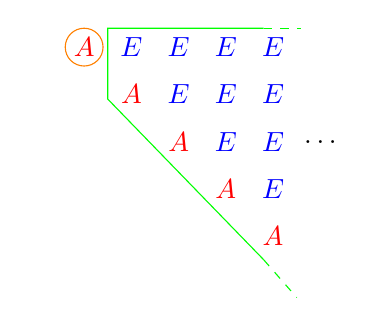
\begin{tikzpicture}[scale = 0.6]
    \foreach \y in {0,...,2}
    {\foreach \x in {\y,...,2}
      \draw (\x+1, -\y) node[color=blue]{$E$} ;
    }
    \foreach \x in {-1,...,3} \draw (\x, -\x-1) node[color=red]{$A$} ;
    \foreach \x in {0,...,3} \draw (\x, -\x)
    node[color=blue]{\textbf{$E$}} ;
    \draw(4,-2) node{$\ldots$};
    
    
%       \draw[color=purple!70]  (2.4, -4.3) --node[auto, swap, left]{$\cut$}
%      (-1.2,-0.6) -- (2.8,-0.6);
%     \draw[color=purple!70, dashed]  (2.8,-0.6) -- (3.6,-0.6);
%     \draw[color=purple!70, dashed]  (2.4,-4.3) -- (3.0,-5);

    \draw[color=orange] (-2,0) node{$\head$} ;
    \draw[color=orange] (-1,0) circle(0.4cm);

    \draw[color=green] (2.8,0.4) -- (-0.5,0.4) -- (-0.5, -1.1) --node[auto, swap, left]{$\tail$}
    (2.8,-4.5)  ; 
    \draw[color=green, dashed] (2.8,0.4) -- (3.6,0.4) ; 
    \draw[color=green, dashed] (2.8,-4.5) -- (3.5,-5.3) ; 


%     \draw[color=orange](0, -0.5) ellipse (12pt and 25pt) ;  
%     \draw[color=orange](1, -1.5) ellipse (12pt and 25pt) ;  
%     \draw[color=orange](2, -2.5) ellipse (12pt and 25pt) ;  
%     \draw[color=orange](3, -3.5) ellipse (12pt and 25pt) ;  
  \end{tikzpicture}\\[-2ex]
  \caption{An infinite triangular matrix over type $A$ and its destructors $\head$ and $\tail$}\label{fig_tri}
 \end{figure}
\end{Long}
% 
 The codata type is specified via two destructors $\head$ and $\tail$, whose types are given in \Cref{tri_rules}.
\begin{Long}
 Given a matrix over type $A$, its $\tail$---obtained by removing the first element on the diagonal, i.e.\ the $\head$ element---can 
 be considered as a trapezium as indicated by the green line in \Cref{fig_tri}, or alternatively, as
 a triangular matrix over type $E\times A$, by bundling the entries of the diagonal with those above as indicated by the orange frames, shown in \Cref{fig:tri_trap}.
 The latter representation is reflected in the type of the destructor $\tail$.
 \begin{figure}[hbt]
  \centering
  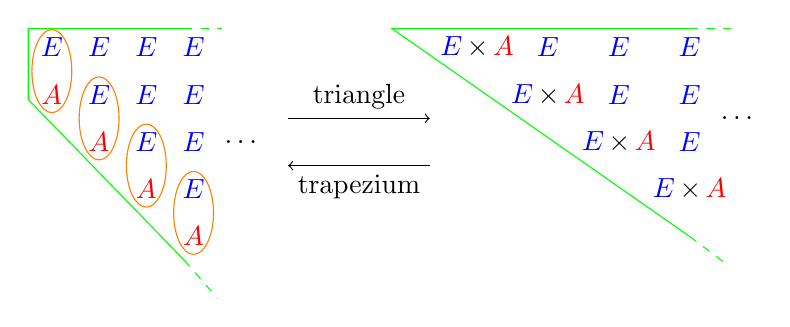
\begin{tikzpicture}[scale = 0.6]
    \foreach \y in {0,...,2}
    {\foreach \x in {\y,...,2}
      \draw (\x+1, -\y) node[color=blue]{$E$} ;
    }
    \foreach \x in {0,...,3} \draw (\x, -\x-1) node[color=red]{$A$} ;
    \foreach \x in {0,...,3} \draw (\x, -\x)
    node[color=blue]{$E$} ;
    \draw(4,-2) node{$\ldots$};

    \foreach \y in {0,...,2}
    {\foreach \x in {\y,...,2}
      \draw (1.5*\x+10.5, -\y) node[color=blue]{$E$} ;
    }
    \foreach \x in {0,...,3} \draw (1.5*\x+9, -\x)
    node{{\color{blue}{$E$}} \hspace*{-.5em} $\times$ \hspace*{-.5em} {\color{red} $A$}} ;
    \draw(14.5,-1.5) node{$\ldots$};
    
    \draw[->] (5,-1.5) to node[swap, auto, above]{triangle}
    (8,-1.5) ; 
    
    \draw[<-] (5,-2.5) to node[swap, auto, below]{trapezium}
    (8,-2.5) ; 

    \draw[color=green] (2.8,0.4) -- (-0.5,0.4) -- (-0.5, -1.1) --
    (2.8,-4.5)  ; 
    \draw[color=green, dashed] (2.8,0.4) -- (3.6,0.4) ; 
    \draw[color=green, dashed] (2.8,-4.5) -- (3.5,-5.3) ; 

    \draw[color=green] (13.5,0.4) -- (7.2,0.4) -- (13.5, -4); 
    \draw[color=green, dashed] (13.5,0.4) -- (14.4,0.4) ; 
    \draw[color=green, dashed] (13.5,-4) -- (14.3,-4.6) ; 

    \draw[color=orange](0, -0.5) ellipse (12pt and 25pt) ;  
    \draw[color=orange](1, -1.5) ellipse (12pt and 25pt) ;  
    \draw[color=orange](2, -2.5) ellipse (12pt and 25pt) ;  
    \draw[color=orange](3, -3.5) ellipse (12pt and 25pt) ;  
  \end{tikzpicture}\\[-2ex]
  \caption{The $\tail$ of a matrix over $A$ is a matrix over $E\times A$ (illustration taken from \parencite{DBLP:conf/types/MatthesP11})}
  \label{fig:tri_trap}
\end{figure}
\end{Long}
\begin{Short}
 Given a matrix over type $A$, its $\tail$---obtained by removing the first element on the diagonal, i.e.\ the $\head$ element---can 
 be considered as a trapezium or, alternatively, as a triangular matrix over type $E\times A$, 
 by bundling the entries of the diagonal with those directly above the diagonal. 
\end{Short}
This change of parameter (from $A$ to $E \times A$) in the type of $\tail$ is why the family $\Tri$ is called \emph{heterogeneous}.

%  As with streams, we denote by $\Tri A$ not only the resulting \emph{setoid} of triangular matrices over $A$, but also its
%  underlying \emph{type}. 
 
 \begin{figure}
 \begin{mdframed}
  
% \section{Rules for $\Tri$ and bisimilarity}\label{tri_rules}

\paragraph*{Rules for $\Tri$}

\begin{description}

 \item[Formation]\hfill \\
 
 \begin{center}
 \def\extraVskip{3pt}
     \def\proofSkipAmount{\vskip.8ex plus.8ex minus.4ex}

         
   \AxiomC{$A : \Set$}
    \UnaryInfC{$\Tri A : \Set$}
     \DisplayProof
 \end{center} 
 
 \item[Elimination]\hfill \\
 

%   \hspace{3ex}

\begin{center}
    \AxiomC{$t : \Tri A$} %\doubleLine
     \UnaryInfC{$\head_A~t : A$}
      \DisplayProof
                        \hspace{3ex}
                                       \AxiomC{$t : \Tri A$}%\doubleLine
                                       \UnaryInfC{$\tail_A~t : \Tri(E\times A)$}
                                       \DisplayProof%
\end{center}
  \item[Introduction]\hfill \\                                     
                       
%           \vspace{1em}             
            
\begin{center}
               \AxiomC{$T : \Set\to\Set$} 
               \AxiomC{$hd : \forall A,TA \to A$} \AxiomC{$tl : \forall A, T A \to T(E\times A)$} %\doubleLine
               \TrinaryInfC{$\corec_T~hd~tl :  \forall A, T A \to \Tri A$}
               \DisplayProof%
\end{center}
                      
%           \vspace{1em}
  \item[Computation]\hfill \\

\begin{center}          
               \AxiomC{$hd : \forall A,TA \to A$} \AxiomC{$tl : \forall A, T A \to T(E\times A)$} %\doubleLine
               \AxiomC{$t : TA$}
               \TrinaryInfC{$\head_T(\corec_A~hd~tl~t) = hd(t)$}
               \DisplayProof
               
               \vspace{1em}
               
               \AxiomC{$hd : \forall A,TA \to A$} \AxiomC{$tl : \forall A, T A \to T(E\times A)$} %\doubleLine
               \AxiomC{$t : TA$}
               \TrinaryInfC{$\tail_T(\corec_A~hd~tl~t) = \corec_A~hd~tl~(tl~t)$}
               \DisplayProof
\end{center}

 \end{description}              
               
\paragraph*{Bisimilarity for $\Tri$}              
 


               
 \begin{description}

 \item[Formation]\hfill \\
 
 \begin{center}
 \def\extraVskip{3pt}
     \def\proofSkipAmount{\vskip.8ex plus.8ex minus.4ex}

         
   \AxiomC{$A : \Set$} \AxiomC{$s, t : \Tri A$}
    \BinaryInfC{$\bisim_A~s~t : \Set$}
     \DisplayProof
 \end{center} 
 
 \item[Elimination]\hfill \\
 

%   \hspace{3ex}

\begin{center}
    \AxiomC{$s, t : \Tri A$} \AxiomC{$p: \bisim_A~s~t$} %\doubleLine
     \BinaryInfC{$\head_A~s = \head_A~t$}
      \DisplayProof
                        \hspace{3ex}
                                       \AxiomC{$s,t : \Tri A$} \AxiomC{$p: \bisim_A~s~t$}%\doubleLine
                                       \BinaryInfC{$\bisim_A (\tail_A~s) (\tail_A~t)$}
                                       \DisplayProof%
\end{center}
  \item[Introduction]\hfill \\                                     
                       
%           \vspace{1em}             
            
\begin{center}
               \AxiomC{$R : \forall A, \Tri A \to \Tri A \to \Set$} \noLine
               \UnaryInfC{$\forall A,\forall~s,t : \Tri A, R~s~t \to \head~s = \head~t$} \noLine
                \UnaryInfC{$\forall  A,\forall~s,t : \Tri A, R~s~t \to R~(\stail~s) (\stail~t)$}  %\doubleLine
               \UnaryInfC{$\forall A,\forall~s,t : \Tri A, R~s~t \to \bisim~s~t$}
               \DisplayProof%
\end{center}

\end{description}
               
 \end{mdframed}
 \caption{Rules for triangular matrices and bisimilarity on them} \label{tri_rules}
\end{figure}
 

\begin{comment}
\begin{figure}[bt]
  \centering

     \def\extraVskip{3pt}
     \def\proofSkipAmount{\vskip.8ex plus.8ex minus.4ex}
    \AxiomC{$t : \Tri~A$} %\doubleLine
     \UnaryInfC{$\head_A~t : A$}
      \DisplayProof
                        \hspace{3ex}
                                       \AxiomC{$t : \Tri~A$}%\doubleLine
                                       \UnaryInfC{$\tail_A~t : \Tri(E\times A)$}
                                       \DisplayProof%
% 
% 
% \vspace{2ex}
% 
 \hspace{3ex}
                                            \def\extraVskip{3pt}
     \def\proofSkipAmount{\vskip.8ex plus.8ex minus.4ex}
    \AxiomC{$t \sim t'$}%\doubleLine
     \UnaryInfC{$\head~t = \head~t'$}
      \DisplayProof
                        \hspace{3ex}
                                       \AxiomC{$t \sim t'$}%\doubleLine
                                       \UnaryInfC{$ \tail~t \sim \tail~t'$}
                                       \DisplayProof   

  \caption{Destructors and bisimilarity for the coinductive family $\Tri$} \label{fig:tri_destructors}
\end{figure}
\end{comment}
% 
% 
  A cosubstitution operation, \enquote{redecoration},
    $ \redec_{A,B} : (\Tri A \to B) \to \Tri A \to \Tri B$
  is defined  through the clauses
% 
  \begin{align} \comp{\redec~f}{\head} := f \quad\text{ and } \quad
                  \comp{\redec~f}{\tail} := \comp{\tail}{\redec~(\extend~f)} \enspace . \label{eq:rest_redec}
    \end{align}
An illustration of the redecoration operation is given in \Cref{fig:redec}, 
taken from the article by \textcite{DBLP:conf/types/MatthesP11}.    
\begin{figure}[tbp]
  \centering
  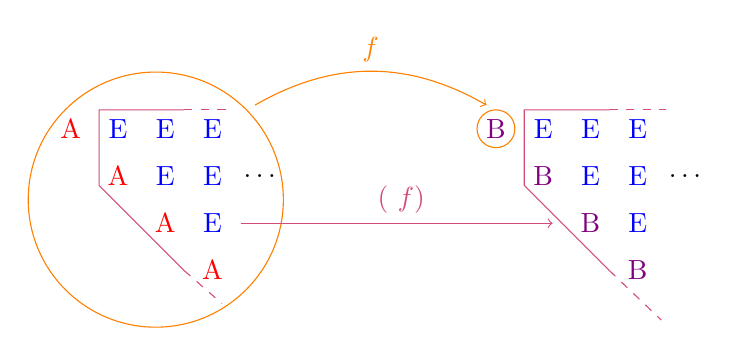
\begin{tikzpicture}[scale = 0.6]
    
    \foreach \y in {0,...,2}
    {\foreach \x in {\y,...,2}
      \draw (\x+1, -\y) node[color=blue]{E} ;
    }
    \foreach \x in {0,...,3} \draw (\x, -\x) node[color=red]{A} ;
    \draw(4,-1) node{$\ldots$};

    \foreach \y in {0,...,2}
    {\foreach \x in {\y,...,2}
      \draw (\x+10, -\y) node[color=blue]{E} ;
    }
    \foreach \x in {0,...,3} \draw (\x+9, -\x) node[color=violet]{B} ;
    \draw(13,-1) node{$\ldots$};
    \draw[color=purple!70]  (2.4, -3) --
    (0.6,-1.2) -- (0.6,0.4) -- (2.4,0.4);
    \draw[color=purple!70, dashed]  (2.4,0.4) -- (3.4,0.4);
    \draw[color=purple!70, dashed]  (2.4,-3) -- (3.2,-3.7);
 
    \draw[color=orange] (1.8,-1.5) circle(2.7cm);

    \draw[color=purple!70]  (11.4, -3) --
    (9.6,-1.2) -- (9.6,0.4) -- (11.4,0.4);
    \draw[color=purple!70, dashed]  (11.4,0.4) -- (12.6,0.4);
    \draw[color=purple!70, dashed]  (11.4,-3) -- (12.5,-4.05);
    
    \draw[color=orange] (9,0) circle(0.4cm);
    
    \draw[->,color = orange] (3.9,0.5) to [bend left] node[auto,
    swap, above]{$f$} (8.8,0.5) ; 

    \draw[->,color = purple!70] (3.6,-2) to node[auto,
    swap, above]{$\redec~(\lift~f)$} (10.2,-2) ; 
    
  \end{tikzpicture}
  \caption{Definition of redecoration (illustration taken from \parencite{DBLP:conf/types/MatthesP11})}
  \label{fig:redec}
\end{figure}

    
Here, the family of functions 
     $\extend_{A,B} : (\Tri A \to B) \to \Tri (E \times A) \to E\times B $
  is suitably defined to account for the change of the type of the argument of $\redec$ when redecorating $\tail~t : \Tri(E\times A)$
  rather than $t : \Tri A$, namely
  \[ \extend(f) := \langle \comp{\head_{E\times A}}{\pr_1(E,A)} , \comp{\cut_A}{f} \rangle \enspace . \]
  An illustration of this operation is given in \Cref{fig:lift}, 
  taken from the article by \textcite{DBLP:conf/types/MatthesP11}.    
  \begin{figure}[tbp]
  \centering
  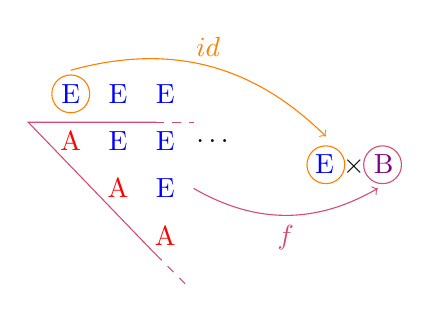
\begin{tikzpicture}[scale = 0.6]
    \foreach \y in {0,...,2}
    {\foreach \x in {\y,...,2}
      \draw (\x+1, -\y) node[color=blue]{E} ;
    }
    \foreach \x in {1,...,3} \draw (\x, -\x) node[color=red]{A} ;
    \draw(4,-1) node{$\ldots$};

     \draw (7,-1.5) node{{\color{blue} E} $\times$ {\color{violet} B}} ;
    \draw[color=orange] (1,0) circle(0.4cm);
    \draw[color=orange] (6.4,-1.5) circle(0.4cm);
    \draw[color=purple!70]  (2.8, -3.4) --
     (0.1,-0.6) -- (2.8,-0.6);
    \draw[color=purple!70, dashed]  (2.8,-0.6) -- (3.6,-0.6);
    \draw[color=purple!70, dashed]  (2.8,-3.4) -- (3.5,-4.1);

    \draw[color=purple!70] (7.6,-1.5) circle(0.4cm);

     \draw[->, color = orange] (1,0.5) to [bend left] node[auto,
     swap, above]{$id$} (6.4,-0.9) ; 
    \draw[->, color = purple!70] (3.6,-2) to [bend right] node[auto,
    swap, below]{$f$} (7.5,-2) ; 
    
  \end{tikzpicture}
  \vspace{-3ex}
  \caption{Definition of lifting (illustration taken from \parencite{DBLP:conf/types/MatthesP11})}
  \label{fig:lift}
\end{figure}
% 
  The auxiliary function $\cut_A : \Tri(E\times A) \to \Tri A$ cuts the upper row of elements in $E$ of a trapezium (equivalently, of a matrix over $E\times A$).
  It is defined corecursively via
% 
  \begin{align*} \comp{\cut}{\head} := \comp{\head}{\pr_2} \quad\text{ and } \quad
                     \comp{\cut}{\tail} := \comp{\tail}{\cut} \enspace . 
      \end{align*}
%       
All the operations are suitably compatible with the bisimilarity relations, so that they can be equipped with the types
  \begin{align*}
    \redec_{A,B} &: \Setoid(\Tri A,\eq B) \to \Setoid(\Tri A,\Tri B ) \\
    \extend_{A,B} &: \Setoid(\Tri A,\eq B) \to \Setoid\bigr(\Tri (E \times A),\eq(E\times B)\bigr) \\
    \cut_A &:  \Setoid(\Tri(E\times A) , \Tri A) \enspace .
  \end{align*}
\end{ex}

\begin{Long}
Note how heterogeneity of the destructor $\tail$ makes the definition of $\redec$ considerably more complicated than that of
the analogous operation $\sredec$ on streams.
\end{Long}

\begin{rem}
 We do not specify any computation rules for bisimilarity, i.e., we think of bisimilarity as a proof-irrelevant notion. 
 Categorically, the lack of such a computation rule amounts to saying that bisimilarity is a \emph{weakly} terminal bisimulation on the respective codata. 
\end{rem}


  
\section{Relative comonads and their morphisms}\label{sec:comonads}

In this section we define the category of \emph{comonads relative to a fixed functor}, and present some examples 
of such comonads and their morphisms.

\emph{Relative monads} were defined by \textcite{DBLP:conf/fossacs/AltenkirchCU10} as a notion of monad-like structure
whose underlying functor is not necessarily an endofunctor. 
An example of relative comonad given in that work is the lambda calculus over finite contexts.


The dual notion is that of a relative \emph{co}monad, more precisely, a comonad relative to some functor $F:\C\to\D$.
Indeed, since the functor underlying a relative comonad is not necessarily endo, one requires an auxiliary functor, which 
\enquote{mediates} between source and target category.
An application of this auxiliary functor is inserted where necessary to make the comonad-like operations and axioms welltyped.

\begin{defn}%[Relative comonad]
 \label{def:rel_comonad}
  Let $F:\C\to\D$ be a functor. A \fat{relative comonad $T$ over $F$} is given by
  \begin{itemize}%\setlength{\itemsep}{\itemizedist}
   \item a map $T:\C_0 \to \D_0$ on the objects of the categories involved;
   \item an operation \[\counit : \forall A : \C_0, \D(TA,FA)\]
   \item an operation \[\cobind: \forall A,B:\C_0, \D(TA,FB) \to \D(TA,TB)\]
  \end{itemize}
   such that the following equations hold:
 \begin{align}
  & \forall A,B:\C_0, \forall f:\D(TA,FB), \comp{\cobind(f)}{\counit_B} = f \\
  & \forall A : \C_0, \cobind(\counit_A) = \id_{TA} \\
  & \forall A,B,C:\C_0, \forall f : \D(TA,FB),\forall g:\D(TB,FC), \notag \\
  &  \qquad    \comp{\cobind(f)}{\cobind(g)} = \cobind(\comp{\cobind(f)}{g}) \enspace ,
 \end{align}
   
  in diagrammatic form:
\[ \begin{xy}
    \xymatrix@C=4em{
                       TA \ar[r]^{\cobind(f)} \ar[rd]_{f}& TB \ar[d]^{\counit_B} \\
                          & FB
    }
    \end{xy}
    \qquad
    \begin{xy}
    \xymatrix{
                       TA \ar@/^1pc/[rd]^{\cobind(\counit_A)} \ar@/_1pc/[rd]_{\id}& \\
                          & TA
    }
   \end{xy}
   \qquad
   \begin{xy}
    \xymatrix@C=4em{
       TA \ar[r]^{\cobind(f)} \ar[rd]_{\cobind(\comp{\cobind(f)}{g})\;\;\;\;}& TB \ar[d]^{\cobind(g)} \\
          & TC .
    }
   \end{xy}
\]
\end{defn}

\begin{Short}
\begin{rem}\label{def:lift}
 \begin{itemize}
  \item Relative comonads over the identity functor are comonads.
  \item Just like relative monads, relative comonads are functorial.
  \item Under some conditions on the functor $F$, one can obtain comonads relative to $F$ from (absolute) comonads on the 
 source category $\C$.
  \item A \emph{weak constructive comonad} as defined by \textcite{DBLP:conf/types/MatthesP11}  is \emph{precisely}
  a comonad relative to the functor $\eq : \Set\to\Setoid$.
 \end{itemize}
\noindent
Details are given in the long version of this article \parencite{trimat_coq}.
\end{rem}
\end{Short}


\begin{Long}
 \Cref{def:rel_comonad} does not mention an action of $T$ on morphisms. Indeed, just like with relative monads, this action is definable rather than part of the definition:
\begin{defn}%[Functoriality for relative comonads]
\label{def:lift}
 Let $T$ be a  comonad relative to $F:\C\to\D$.
 For $f : \C(A,B)$ we define
  \[ T(f) := \cobind(\comp{\counit_A}{Ff}) : \D(TA,TB) \enspace .\] 
 The functor properties are easily checked.
\end{defn}

\begin{rem}
 It follows from the comonadic axioms that
 counit and cobind are natural transformations with respect to the functoriality defined in \Cref{def:lift}:
 \begin{align*}
     \counit &: T \to F : \C\to \D \\
     \cobind &: \D(T\_, F\_) \to \D(T\_, T\_) : \C^{\text{op}} \times \C \to \Ens \enspace .
 \end{align*}

\end{rem}


\end{Long}

\begin{Long}
Comonads relative to the identity functor are exactly (traditional) comonads.
\end{Long}



\begin{Long}
We obtain a comonad relative to $F:\C\to\D$ from a comonad on the category $\C$ by composing $M$ with $F$:
\begin{ex}[Relative comonads from comonads]\label{ex_relcom_from_com}
  Let $F : \C \to \D$ be a fully faithful functor and $(M,\counit,\cobind)$ be a (traditional) comonad (in Kleisli form) on $\C$.
  We define a comonad $FM$ relative to $F$ by setting:
  \begin{itemize}\setlength{\itemsep}{\itemizedist}
   \item $FM(A) := F(MA)$;
   \item $\counit^{FM}_A := F(\counit^M_A) : \D(FMA,FA)$;
   \item $\cobind^{FM}_{A,B} (f) := F\bigl(\cobind^M_{A,B}(F^{-1}f)\bigr)$.
  \end{itemize}
  The proof of the axioms of a relative comonad is immediate.
\end{ex}

The other way round does not require any conditions on the functor $F$:
\begin{ex}[Relative comonads from comonads II]\label{ex_relcom_from_com_on_target}
    Let $F : \C \to \D$ be a functor and $(M,\counit,\cobind)$ be a (traditional) comonad (in Kleisli form) on $\D$.
  We define a comonad $MF$ relative to $F$ by setting:
  \begin{itemize}\setlength{\itemsep}{\itemizedist}
   \item $MF(A) := M(FA)$;
   \item $\counit^{MF}_A := \counit^M_{FA} : \D(MFA,FA)$;
   \item $\cobind^{MF}_{A,B} (f) := \cobind^M_{FA,FB}(f) : \D(MFA,MFB)$ for $f : \D(MFA,FB)$.
  \end{itemize}
  The proof of the axioms of a relative comonad is immediate.
\end{ex}


\end{Long}

The next examples concern the codata type families presented in \Cref{sec:tri}.

\begin{ex}[Streams]\label{ex_stream_comonad}
  The codata type family $\stream : \Set \to \Setoid$ of \Cref{ex_stream} is equipped with a structure of a comonad relative to the functor 
  $\eq : \Set \to \Setoid$ with
   $\counit_A := \shead_A$ and
   $\cobind_{A,B} := \sredec_{A,B}$.
\end{ex}

\begin{Long}
\begin{rem}
 Instead of considering $\stream$ as a relative comonad from $\Set$ to $\Setoid$, it could be considered as a traditional comonad on the 
 category $\Setoid$, propagating the equivalence relation on the base type, say $A$, to $\stream A$.
 The relative point of view can then be recovered as an instance of \Cref{ex_relcom_from_com_on_target}.
\end{rem}
\end{Long}


\begin{Long}

\begin{ex}[Trees]\label{ex_tree_comonad}
 Fix a type $B$. Analogously to \Cref{ex_stream_comonad}, the map $A \mapsto \Tree_B(A)$ of \Cref{ex_trees}
 is equipped with a structure of a comonad relative to $\eq: \Set\to\Setoid$.
\end{ex}

\end{Long}

\begin{ex}[Infinite triangular matrices]\label{ex:tri_comonad}
  The codata type family $\Tri : \Set \to \Setoid$ of \Cref{ex_tri} is equipped with a structure of a comonad relative to the functor 
  $\eq : \Set \to \Setoid$ with
   $\counit_A := \head_A$ and
   $\cobind_{A,B} := \redec_{A,B}$.
\end{ex}

\begin{Long}
\begin{rem}
  A \emph{weak constructive comonad} as defined by \textcite{DBLP:conf/types/MatthesP11} to characterize the codata type $\Tri$
  and redecoration on it, is \emph{precisely}
  a comonad relative to the functor $\eq : \Set\to\Setoid$.
\end{rem}
\end{Long}

\begin{Long}
\begin{rem}[Comonads into cartesian closed categories]
 With the notations of \Cref{def:rel_comonad}, suppose that the category $\D$ is cartesian closed, i.e. that $\D$ has
 internal hom-objects. This is the case, e.g., for the category $\Setoid$ of setoids.
 The cobind operation of a relative comonad into $\D$ might then be defined to be a family of arrows in $\D$,
  \begin{equation}\cobind_{A,B} : \underline{\D}(TA,FB) \to \underline{\D}(TA,TB) \enspace . \label{eq_enriched}\end{equation}
 The comonads $\stream$ (cf.\ \Cref{ex_stream_comonad}) and $\Tri$ (cf.\ \Cref{ex_tree_comonad}) are comonads with such a cobind operation. In these two cases, this \enquote{enriched} definition of the cobind operation given in \Cref{eq_enriched} encodes a higher-order 
 compatibility of cosubstitution with bisimilarity, namely that cosubstitution with two extensionally bisimilar functions
 yields extensionally bisimilar functions.
\end{rem}
\end{Long}



The notion of relative comonad captures many properties of $\stream$ resp.\ $\Tri$ and cosubstitution on them, in particular the interplay
of cosubstitution with the destructors $\shead$ resp.\ $\head$ via the first two axioms.
In order to  capture the interplay 
of cosubstitution  with the destructor $\stail$ (for streams) resp.\ $\tail$ (for infinite triangular matrices), we develop the notion of \emph{comodule over a relative comonad}
 in \Cref{sec:comodules}. 




\emph{Morphisms of relative comonads} are families of morphisms that are compatible with the comonadic structure:

\begin{defn}%[Morphism of relative comonads]
\label{def:comonad_morphism}
 Let $T$ and $S$ be comonads relative to a functor $F : \C \to \D$. A \fat{morphism of relative comonads} $\tau : T \to S$
  is given by a family of morphisms \[\tau_A : \D(TA,SA)\] such that the following diagrams commute: 
  for any $A : \C_0$ (first diagram), and, for any $A,B : \C_0$ and $f : \D(SA,FB)$ (second diagram),
%      \[  \counit^T_A = \comp{\tau_A}{\counit^S_A} \]
     
\[ \begin{xy}
    \xymatrix {
                       TA \ar[r]^{\tau_A} \ar[rd]_{\counit^T_A}  &   SA \ar[d]^{\counit^S_A}\\
                            &    FA
   }
   \end{xy}
% 
% 
%   
%    \[  \comp{\cobind^T(\comp{\tau_A}{f})}{\tau_B} = \comp{\tau_A}{\cobind^S(f)} \enspace . \]
% 
\qquad
\begin{xy}
     \xymatrix@C=6em{
                     TA \ar[d]_{\tau_A}   \ar[r]^{\cobind^T(\comp{\tau_A}{f})} & TB \ar[d]^{\tau_B}\\
                     SA \ar[r]_{\cobind^S(f)} & SB .
     }  
   \end{xy}
\]

\end{defn}

Relative comonads over a fixed functor $F$ and their morphisms form a category $\RComonad(F)$ with the identity and composition operations given pointwise.

\begin{rem}
A morphism $\tau : T\to S$ of relative comonads over a functor $F:\C\to\D$ is  \emph{natural}
with respect to the functorial action of \Cref{def:lift}.
\end{rem}

\begin{Long}

\begin{ex}[\Cref{ex_relcom_from_com} continued]\label{ex_relcom_from_com_morphism}
 Let $M$ and $M'$ be two monads on $\C$, and let $\tau : M \to M'$ be a comonad morphism. 
 The family of morphisms \[F\tau_A := F(\tau_A) : FMA \to FM'A\] constitutes a morphism of 
 relative comonads $F\tau : FM\to FM'$.
\end{ex}


\begin{rem}
 The definitions given in \Cref{ex_relcom_from_com} and \Cref{ex_relcom_from_com_morphism} yield a functor from 
 comonads on $\C$ to comonads relative to $F:\C\to\D$. 
 If $F$ is a right adjoint with left adjoint $L$, $L\dashv F$, then postcomposing a comonad $T$ relative to $F$ with the functor $L$
 yields a monad on $\C$. Again, this map extends to morphisms.
 The two functors between categories of monads thus defined are again adjoints.
 Writing down the details is lengthy but easy.
 
%  For instance, in a type theory with quotients, such as the \emph{Univalent Foundations} a.k.a.\ \emph{Homotopy Type Theory}
%  \parencite{hottbook}, the functor \enquote{quotient} from setoids to types is left adjoint to the fully faithful 
%  functor $\eq: \Set\to\Setoid$, thus above construction is applicable.
\end{rem}

\end{Long}


An example of comonad morphism is given by the \emph{diagonal} map which extracts the diagonal of an infinite triangular matrix (over type $A$),
yielding a stream over $A$:

\begin{ex}\label{ex_diag}
We define a morphism of relative comonads $\diagonal : \Tri \to \stream$ as follows.
Given a matrix $t : \Tri A$, its diagonal is a stream $\diagonal_A~t : \stream A$.
The map $\diagonal_A$ is defined via the clauses
\begin{align*} \comp{\diagonal_A}{\shead} := \head \quad\text{ and } \quad %\notag\\
                  \comp{\diagonal_A}{\stail} := \comp{\comp{\tail}{\cut}}{\diagonal_A} \enspace . %\label{eq:diag}
    \end{align*}
\end{ex}


\begin{Long}

\begin{rem}[Non-examples]
 The family of destructors $\stail_A : \stream A \to \stream A$  
 does \emph{not} satisfy the axioms for a morphism of relative comonads $\stream\to\stream$.
 
 Similarly, while the map $A \mapsto \Tri(E\times A)$ inherits the structure of a relative comonad (see \Cref{product_comonad}),
 the family $\tail_A : \Tri A \to \Tri(E \times A)$  does \emph{not} constitute a comonad morphism
 of type $\Tri \to \Tri(E \times \_)$.
%  One can, however, equip the functor given by precomposing $\Tri$ with \enquote{product with $E$}, i.e.\
%  $A \mapsto \Tri (E\times A)$, with a structure of relative comonad, induced by that
%  on $\Tri$, cf.\ \Cref{product_comonad}.
\end{rem}

Let $\C$ be a category with products and $E:\C_0$ be an object of $\C$.
The following definition shows how a relative comonad $T$ with domain category $\C$ gives rise to a relative comonad with underlying object map
$A \mapsto T(E\times A)$.
We shall not make use of this definition in what follows: indeed, in \Cref{sec:coalgebras_for_tri} we consider the map $A\mapsto T(E\times A)$
as a \emph{comodule} over $T$, rather than a comonad. The below definition may thus be skipped by the reader.

\begin{defn}\label{product_comonad}
  Let $T$ be a comonad relative to a product-preserving functor $F:\C\to\D$ between categories with finite products,
  and let $E:\C_0$ be a fixed object of $\C$.
 The map $A\mapsto T(E\times A)$ inherits the structure of a comonad relative to $F$ from $T$: the 
 counit is defined as
   \[ \counit_A := \comp{T(\pr_2(E,A))}{\counit^T_{A}} \]
  and the cobind operation as
   \begin{align*} 
            \cobind_{A,B} : \D\bigl(T(E\times A),FB\bigr) &\to \D\bigl(T(E\times A),T(E\times B)\bigr) \\
              f &\mapsto  \cobind^T(\extend'~f)
   \end{align*}
  with $\extend'$ defined as 
  \begin{align*} \extend' : \D\bigl(T(E\times A),FB\bigr) &\to \D\bigl(T(E\times A), F(E\times B)\bigr) \enspace , \\ 
                                            f & \mapsto \comp{\langle \comp{T(\pr_1)}{\counit^T_E}, f \rangle}{{\phi^{F}_{E,B}}^{-1}} \enspace .
  \end{align*}
\end{defn}

\end{Long}



\section{Comodules over relative comonads}\label{sec:comodules}

In this section we develop the notion of \emph{comodule over a relative comonad}, dualizing the notion of module over a relative monad \parencite{ahrens_relmonads}.

\begin{defn}%[Comodule over relative comonad]
\label{def:comodule}
 Let $T$ be a comonad relative to $F:\C\to\D$, and let $\E$ be a category.
 A \fat{comodule over T towards $\E$} consists of
   \begin{itemize}\setlength{\itemsep}{\itemizedist}
   \item a map $M:\C_0 \to \E_0$ on the objects of the categories involved and
   \item an operation \[\mcobind: \forall A,B:\C_0, \D(TA,FB) \to \E(MA,MB)\] such that the following equations hold:
 \begin{align}
 &  \forall A : \C_0, \mcobind(\counit_A) = \id_{MA} \\
 & \forall A,B,C:\C_0, \forall f : \D(TA,FB),\forall g:\D(TB,FC), \notag\\
 &   \qquad      \comp{\mcobind(f)}{\mcobind(g)} = \mcobind(\comp{\cobind(f)}{g}) \enspace ,
 \end{align}
  in diagrammatic form:
\[
    \begin{xy}
    \xymatrix{
                       MA \ar@/^1pc/[rd]^{\mcobind(\counit_A)} \ar@/_1pc/[rd]_{\id}& \\
                          & MA
    }
   \end{xy}
   \qquad
   \begin{xy}
    \xymatrix@C=4em{
       MA \ar[r]^{\mcobind(f)} \ar[rd]_{\mcobind(\comp{\cobind(f)}{g})\;\;\;\;\;}& MB \ar[d]^{\mcobind(g)} \\
          & MC .
    }
   \end{xy}
\]  
  
  
  \end{itemize}

\end{defn}




Every relative comonad constitutes a comodule over itself, the \emph{tautological} comodule:

\begin{defn}[Tautological comodule]
\label{def:tautological_comodule}
  Given a comonad $T$ relative to $F:\C\to\D$, the map $A \mapsto TA$ yields a comodule over $T$ 
  with target category $\D$, the \textbf{tautological comodule} of $T$, also called $T$.
  The comodule operation is given by
    $  \mcobind^T(f) := \cobind^T(f)$. 
\end{defn}




\begin{Long}
Similarly to relative comonads, comodules over these are functorial:
\begin{defn}[Functoriality for comodules]
\label{def:comodule_lift}
 Let $M : \RComod(T,\E)$ be a comodule over $T$ towards some category $\E$. For $f : \C(A,B)$ we define
  \[ M(f) := \mcobind(\comp{\counit_A}{Ff}) .  \]
\end{defn}
\end{Long}

A more interesting example of comodule is given by the functor that maps a type $A$ to the setoid $\Tri(E\times A)$
for some fixed type $E$:
\begin{ex}\label{ex_tri_prod_comod}
   The map $A \mapsto \Tri(E\times A)$ is equipped with a comodule structure over the relative comonad $\Tri$ by
   defining the comodule operation $\mcobind$ as (cf.\ \Cref{ex_tri})
     \[ \mcobind_{A,B} (f) := \redec (\extend~f) \enspace . \]
\end{ex}

We later generalize \Cref{ex_tri_prod_comod}---precomposition with a product---to more general relative comonads over suitable categories.
However, this requires an axiomatization of the $\extend$ operation, more precisely of an important building block of it, the
$\cut$ operation.

A \emph{morphism of comodules} is given by a family of morphisms that is compatible with 
the comodule operation:

\begin{defn}[Morphism of comodules]
\label{def:morphism_of_comodules}
 Let $M$ and $N : \C \to \E$ be comodules over the comonad $T$ relative to  $F:\C \to \D$.
 A \fat{morphism of comodules} from $M$ to $N$ is given by a family of morphisms 
   \[ \alpha_A:\E(MA,NA) \]
 such that for any $A,B:\C_0$ and $f : \D(TA,FB)$ one has
 \[\comp{\mcobind^M(f)}{\alpha_B} = \comp{\alpha_A}{\mcobind^N(f)} \enspace, \]
 in diagrammatic form
 \[
  \begin{xy}
   \xymatrix@C=6em{
     MA  \ar[r]^{\mcobind^M(f)}  \ar[d]_{\alpha_A} & MB \ar[d]^{\alpha_B} \\
     NA  \ar[r]_{\mcobind^N(f)}  & NB.
   }
  \end{xy}
 \]

\end{defn}

The following examples are the motivating ones for us to consider comodule and their morphisms:

 \begin{ex}\label{ex_tail_comodule}
  The family of destructors $\stail_A : \stream A \to \stream A$, indexed by a type $A$, is the carrier of a morphism of tautological comodules (over the relative comonad $\stream$),
  \[ \stail : \stream \to \stream \enspace . \]
 \end{ex}

\begin{ex}\label{ex:tail_comodule}
 The family of destructors $\tail_A : \Tri A \to \Tri(E\times A)$, indexed by a type $A$, of \Cref{ex_tri} is a morphism of comodules over the comonad $\Tri$ 
  from the tautological comodule  $\Tri$ to the comodule $\Tri(E\times \_)$ as defined in \Cref{ex_tri_prod_comod},
  \[ \tail : \Tri \to \Tri(E\times \_) \enspace . \]
\end{ex}

Composition and identity of comodule morphisms happens pointwise. We thus obtain a category $\RComod(T,\E)$
 of comodules
over a fixed comonad $T$, towards a fixed category $\E$.



\begin{Long}
\begin{rem}
  The family of morphisms constituting a comodule morphism is actually natural with respect to the functoriality 
  defined in \Cref{def:comodule_lift}.
\end{rem}
\end{Long}

Given a morphism of comonads, we can \enquote{transport} comodules over the source comonad to comodules over the target comonad:


\begin{defn}[Pushforward comodule]
\label{def:pushforward_comodule} 
  Let $\tau : T\to S$ be a morphism of comonads relative to a functor $F : \C \to \D$, and let furthermore $M$ be a 
  comodule over $T$ towards a category $\E$. We define the \fat{pushforward comodule} $\tau_*M$ to be the comodule over $S$ given by
  $  \tau_*M(A) := MA $
  and, for $f : \D(SA,FB)$,
   \[ \mcobind^{\tau_*M}(f) := \mcobind^M(\comp{\tau_A}{f}) : \E(MA,MB) \enspace . \]
   
  \noindent
  Pushforward is functorial: if $M$ and $N$ are comodules over $T$ with codomain category $\E$, and $\alpha : M\to N$ is 
    a morphism of comodules, then we define 
     $\tau_*\alpha : \tau_*M \to \tau_*N$
    as the family of morphisms
     $ (\tau_*\alpha)_A := \alpha_A$.
  It is easy to check that this is a morphism of comodules (over $S$) between $\tau_*M$ and $\tau_*N$.
  Pushforward thus yields a functor \[\tau_*:\RComod(T,\E) \to \RComod(S,\E) \enspace . \]
\end{defn}


As presented in \Cref{def:tautological_comodule}, every relative comonad induces a comodule over itself.
This extends to morphisms of relative comonads:

\begin{defn}%[Morphism of comonads induces morphism of comodules]
\label{def:induced} 
  Let $\tau : T\to S$ be a morphism of comonads relative to $F : \C \to \D$.
  Then $\tau$ gives rise to a morphism of comodules over $S$ from the pushforward of the tautological comodule
  of $T$ along $\tau$ to the tautological comodule over $S$,
  \[ \induced{\tau} : \tau_*T \to S \enspace , \quad \induced{\tau}_A := \tau_A \enspace . \]
\end{defn}




\section{Terminality for streams and infinite triangular matrices}\label{sec:coalgebras_for_tri}

In this section, we define a notion of \enquote{model} for the signatures of streams and triangular matrices,
respectively. We then show that the codata types $\stream$ and $\Tri$ constitute the terminal object in
the respective category of models.


This terminal semantics result is hardly surprising; however, it is still interesting as it characterizes not only the codata types themselves,
 but also the respective bisimilarity relations and comonadic operations on them, via a universal property.



\begin{Long}
\subsection{Models for $\stream$}

We first consider the homogeneous codata type of streams.
\end{Long}

\begin{defn}[Category of models for $\stream$]
 \label{cat_stream}
  A \fat{model for $\stream$} is given by a pair $(S,t)$ 
  consisting of
  \begin{itemize}
   \item a comonad $S$ relative to $\eq : \Set \to \Setoid$ and
   \item a morphism $t$ of tautological comodules over $S$, 
                   \[t : S \to S \enspace . \]
  \end{itemize}
  A \fat{model morphism} $(S,t) \to (S',t')$ is given by a comonad morphism $\tau : S \to S'$ such that
     $ \comp{\tau_*t}{\induced{\tau}} = \comp{\induced{\tau}}{t'}$, in diagrammatic form,
 \[
  \begin{xy}
   \xymatrix{
                  S \ar[r]^{\tau_*t} \ar[d]_{\induced{\tau}} & S \ar[d]^{\induced{\tau}}\\
                  S' \ar[r]_{t'} & S' .
   }
  \end{xy}
 \]
  Note that the above diagram is a diagram in the category $\RComod(S', \Setoid)$. 
  
  This defines a category, with composition and identity inherited from those of comonad morphisms.

\end{defn}

In the introduction, we mentioned a more traditional notion of \enquote{model} for a signature of a coinductive data type, 
namely that of a coalgebra of some endofunctor. The relationship is as follows:

\begin{rem}[Coalgebras for streams: forgetting cosubstitution]\label{rem:coalg_stream}
 We define 
  \begin{align*}  F: [\Set,\Setoid] &\to [\Set,\Setoid]  \enspace , \\
                      F(G)(A) &:= \eq(A) \times G(A) \enspace .
  \end{align*}
  Then we have a forgetful functor from models for streams (in the sense of \Cref{cat_stream}) to coalgebras of $F$ which, intuitively, forgets the cosubstitution structure.
  Indeed, given a model $(S,t)$, the comonad $S$ is, in particular, a functor $S:\Set\to\Setoid$ which constitutes the carrier of 
  a coalgebra of $F$: the coalgebra structure, as a map into a product, 
  is assembled from the counit of $S$ as the first component, and the comodule morphism $t:S\to S$, which
  is a natural transformation $t : S \to S$ as the second component.
\end{rem}
  
  The reason why we consider the richer notion of model (as compared to coalgebras) is that we want the objects of 
  our category---and thus in particular the terminal object---to be equipped with a well-behaved \enquote{cosubstitution} operation.
  It is this cosubstitution operation which is modeled by the comonad and comodule structure, and which is forgotten by 
  the forgetful functor $U$ defined above.

  
  The category of models for $\stream$ has a terminal object:
  
\begin{thm}\label{thm_stream_terminal}
 The pair $(\stream, \stail)$, where $\stream$ is considered as a relative comonad and $\stail$ as
 a morphism of comodules, is the terminal object in the category of models of \Cref{cat_stream}.
\end{thm}

\begin{Long}
More precisely, the aforementioned theorem says that the rules given in \Cref{stream_rules} allow to prove that
the category of models defined in \Cref{cat_stream} has a terminal object.
The proof of \Cref{thm_stream_terminal} being essentially the same as that of \Cref{ex:final_sem_tri}, we omit the former.
However, a mechanized proof can be found in our \coq library, see \Cref{sec:formal}.
\end{Long}


The property of being terminal can be used to specify a map into streams, by equipping some comonad $S$ relative to $\eq:\Set\to\Setoid$
with the structure of a model for streams, that is, with a comodule morphism $S\to S$.
We do so for the comonad $\Tri$:

\begin{ex}
  We equip the relative comonad $\Tri$ with the structure of a model for $\stream$ by defining a 
  morphism of tautological comodules over $\Tri$, given by
   \[ t^{\diagonal} := \comp{\tail}{\cut}  : \Tri \to \Tri \enspace . \]
  It follows that the resulting terminal model morphism
   \[(\Tri, t^{\diagonal}) \to (\stream, \stail)\] has as underlying morphism of relative comonads the one defined in \Cref{ex_diag}.
\end{ex}

\begin{Long}
 
\begin{rem}
 Fix a type $B$. A result analogous to \Cref{thm_stream_terminal} holds for trees $\Tree_B$ of \Cref{ex_tree_comonad}. 
 We refrain from giving a precise statement of this result.
\end{rem}

\end{Long}

\begin{Long}
\subsection{Models for $\Tri$}
\end{Long}

In analogy to the definition of models for the signature of streams, one would like to define
a model for the signature of $\Tri$ as a pair $(T,r)$ of a comonad $T$ relative to $\eq : \Set \to \Setoid$ and 
a morphism of comodules $r : T \to T(E\times \_)$. 
It turns out that in this way, one does not obtain the right auxiliary function $\cut$ for what is
supposed to be the \emph{terminal} such model, the pair $(\Tri,\tail)$, where $\cut$ is used to define the comodule $\Tri(E\times \_)$.
As a remedy, we define a model to come equipped with a specified operation analogous to $\cut$, and some laws governing
the behavior of that operation:




\begin{defn}%[Relative comonad with cut]
\label{def:rel_comonad_with_cut}
 Let $\C$ and $\D$ be categories with binary products and $F:\C\to\D$ a product-preserving functor. Let $E:\C_0$ be a fixed object of $\C$.
 We define a \fat{comonad relative to $F$ with cut relative to $E$} to be a comonad $T$ relative to $F$ together with a $\cut$ operation 
    \[ \cut : \forall~A:\C_0, T(E\times A) \to TA \]
%   
 satisfying the axioms
  \begin{itemize}
%    \item $\forall~A:C_0, \comp{\cut_A}{\counit_A} = \comp{\counit_{E\times A}}{F(\pr_2(E,A))}$;
   \item $\forall~A:C_0, \comp{\cut_A}{\counit_A} = \comp{T(\pr_2(E,A))}{\counit_{A}}$;
   \item $\forall~A~B:C_0,\forall~f:\D(TA,FB), \comp{\cut_A}{\cobind(f)} = \comp{\cobind(\extend~f)}{\cut_B}$,
  \end{itemize}
that is,
\[
 \begin{xy}
  \xymatrix@C=5em{
                T(E\times A) \ar@<1ex>[r]^-{T(\pr_2(E,A))} \ar@<-1ex>[r]_-{\cut_A} & TA \ar[r]^{\counit_A} & FA
  }
 \end{xy}
 \quad\text{ and } \quad
 \begin{xy}
  \xymatrix@C=5em{
	      T(E\times A) \ar[r]^{\cobind(\extend~f)} \ar[d]_{\cut_A} & T(E\times B) \ar[d]^{\cut_B} \\
	      TA \ar[r]_{\cobind(f)} &  TB 
  }
 \end{xy}
\]


  \noindent
  where, for $f:\D(TA,FB)$, we define $\extend(f) : \D\bigl(T(E\times A),F(E\times B)\bigr)$ as
       \[ \extend(f) := \comp{\comp{\langle T(\pr_1) , \cut \rangle}{(\counit_E\times f)}}{{\phi^{F}_{E,B}}^{-1}} \enspace . \]
  
\end{defn}

Morphisms of comonads with cut are morphisms of comonads that are compatible with the respective $\cut$ operations:

\begin{defn}%[Morphism of comonads with cut]
\label{def:morphism_comonad_cut}
 Let $(T,\cut^T)$ and $(S,\cut^S)$ be two comonads relative to a functor $F$ with cut relative to $E$ as in \Cref{def:rel_comonad_with_cut}.
 A \fat{morphism of comonads with cut} is a comonad morphism $\tau$ between the underlying comonads as in \Cref{def:comonad_morphism} that 
 commutes suitably with the respective $\cut$ operations, i.e.\ for any $A : \C_0$,
  $\comp{\tau_{E \times A}}{\cut^S_A}  = \comp{\cut^T_A}{\tau_A}$:
\[
 \begin{xy}
  \xymatrix@C=4em{
                 T(E\times A)   \ar[r]^-{\cut^T_A} \ar[d]_{\tau_{E \times A}}  & TA \ar[d]^{\tau_{A}}\\
                 S(E \times A)  \ar[r]_-{\cut^S_A}   & S A.
  }
 \end{xy}
\]

\end{defn}


Comonads with cut relative to a fixed functor $F:\C\to\D$ and $E:\C_0$ form a category $\RComonadWC(F,E)$.
There is a forgetful functor from $\RComonadWC(F,E)$ to $\RComonad(F)$.
Conversely, any comonad $T$ relative to a suitable functor can be equipped with a $\cut$ operation, using functoriality of $T$.
%
\begin{Short}
 Details are given in the long version of this article.
\end{Short}

\begin{Long}
\begin{rem}[Canonical $\cut$ operation]\label{canonical_cut}
 Any comonad $T$ relative to a product-preserving functor $F:\C\to\D$  can be equipped with a $\cut$ operation relative to 
 $E:\C_0$ satisfying the properties of \Cref{def:rel_comonad_with_cut} by setting
   \[ \ccut_A := \cut_A := T\bigl(\pr_2(E,A)\bigr) \enspace . \]
 (The extra \enquote{c} of $\ccut$ stands for \enquote{canonical}.)
 It follows from the axioms of comonad morphism that a comonad morphism $\tau : T\to S$ satisfies the equation of \Cref{def:morphism_comonad_cut} 
 for the  operations $\ccut^T$ and $\ccut^S$ thus defined. The morphism $\tau$ hence constitutes a morphism of comonads with cut from $(T,\ccut^T)$ to $(S,\ccut^S)$.
 We thus obtain a functor 
 \[ \ccut_{F,E} : \RComonad(F) \to \RComonadWC(F,E)\]
 from relative comonads over $F$ to relative comonads over $F$ with cut relative to a fixed object $E:\C_0$ given on 
 objects by $T\mapsto (T,\ccut^T)$.
\end{rem}

The functor $\ccut_{F,E}$, followed by the forgetful functor, yields the identity. We can thus view
relative comonads with cut as a generalization of relative comonads.
\end{Long}

\begin{Long}
Our prime example of relative comonad comes with a $\cut$ operation that is \emph{not} the canonical one:
\end{Long}

\begin{ex}%[$\cut$ for $\Tri$]
\label{def:cut_for_tri}
  The relative comonad $\Tri$ from \Cref{ex:tri_comonad}, together with the $\cut$ operation defined in \Cref{ex_tri}, 
  is a comonad with cut as in \Cref{def:rel_comonad_with_cut}.
\end{ex}





Given a comodule $M$ over a relative comonad $T$ with cut, we define a comodule over $T$ obtained by precomposition of $M$ with
\enquote{product with a fixed object $E$}:


\begin{defn}%[Precomposition with product]
\label{def:product_in_context}
 Suppose $F:\C\to\D$ is a product-preserving functor, and $T$ is a comonad relative to $F$ with a $\cut$ operation 
 relative to $E:\C_0$ as in \Cref{def:rel_comonad_with_cut}.
 Given a comodule $M$ over $T$,  \fat{precomposition with} \enquote{\fat{product} with $E$}
 gives a comodule 
   \[ M(E\times\_) : A \mapsto M(E\times A) \] over $T$.
 The comodule operation is induced by that of $M$ by 
 \begin{align*} \mcobind^{M(E\times\_)}_{A,B} : \D(TA,FB)&\to \E\bigl(M(E\times A), M(E\times B)\bigr) \enspace ,\\ 
                                                      f &\mapsto \mcobind^M_{E\times A,E\times B}(\extend(f)) \enspace ,
  \end{align*}                                        
where the $\extend$ operation is the one defined in \Cref{def:rel_comonad_with_cut}.
 
 Furthermore, given two comodules $M$ and $N$ over $\T$ with target category $\E$, and a comodule morphism $\alpha : M \to N$,  
 the assignment \[ \alpha(E \times \_)_A := \alpha_{E\times A} \] defines a comodule morphism 
  $\alpha(E\times \_) : M(E\times \_) \to N(E\times \_) $.

\begin{Long}
  \noindent
  We thus obtain an endofunctor on the category of comodules over $T$ towards $\E$,
   \[ M \mapsto  M (E\times \_) : \RComod(T,\E) \to \RComod(T,\E) \enspace . \]
\end{Long}
\end{defn}



\begin{rem}[Pushforward commutes with product in context]\label{rem:prod_pullback_commute}
 Note that the constructions of \Cref{def:product_in_context} and \Cref{def:pushforward_comodule} commute:
 we have an isomorphism of comodules 
  \[     \tau_*(M(E\times \_)) \cong (\tau_*M)(E \times \_)        \]
 given pointwise by identity morphisms.
\end{rem}


\begin{Long}

It directly follows from the definition that the cut operation of any comonad $T$ with cut 
constitutes a comodule morphism $\cut : T(E\times \_) \to T$.
We can thus restate the definition of a morphism of comonads with cut as in \Cref{def:morphism_comonad_cut} by asking the following diagram 
of comodule morphisms (in the category $\RComod(S,\D)$) to commute
(where in the upper left corner we silently add an isomorphism as in \Cref{rem:prod_pullback_commute}):
 \[ \begin{xy}
       \xymatrix{  **[l] \tau_*T(E\times \_ )  \ar[r]^{\tau_*(\cut^T)} \ar[d]_{\induced{\tau}(E\times \_)}  &  **[r] \tau_*T \ar[d]^{\induced{\tau}} \\
                   **[l]  S (E\times \_ ) \ar[r]_{\cut^S}  &  **[r] S  \enspace .
        }
      \end{xy}
   \]

\end{Long}



\begin{Long}
The construction of \Cref{def:product_in_context} yields a categorical characterization of the $\tail$ destructor---%
more precisely, of its behavior with respect to cosubstitution as in \Cref{eq:rest_redec}---via the notion of comodule morphism:

% TODO: this is bs
\begin{ex}\label{ex:tail_comodule_alternative}
\Cref{def:product_in_context} is an axiomatization of \Cref{ex:tail_comodule}:
the relative comonad $\Tri$ is a relative comonad with cut, and 
the family of destructors $\tail_A : \Tri A \to \Tri (E\times A)$ constitutes a morphism of comodules
\[ \tail : \Tri \to \Tri (E \times \_ ) \]
from the tautological comodule $\Tri$ to the composed comodule $\Tri (E\times \_)$ (obtained by precomposing the tautological comodule $\Tri$
with \enquote{product with $E$} as defined in \Cref{def:product_in_context}).
  
\end{ex}
\end{Long}


The axiomatization of the cut operation now allows us to define models for the signature of infinite triangular matrices:

\begin{defn}[Models for infinite triangular matrices]
\label{def:cat_tri}
   Let $E:\Set$ be a fixed type.
   Let $\mathcal{T} = \mathcal{T}_E$ be the category of \fat{models for infinite triangular matrices} where an object is a pair $(T,\tail^T)$ consisting of
   \begin{itemize}
    \item a comonad $T$ over the functor $\eq:\Set\to\Setoid$ with $\cut$ relative to $E$ and
    \item a morphism $\tail^T$ of comodules over $T$ of type $T \to T(E\times \_)$
   \end{itemize}
   such that for any set $A$,
    $ \comp{\cut^T_A}{\tail^T_A} = \comp{\tail^T_{E\times A}}{\cut^T_{E\times A}}$.
    
 \begin{Long}
   The last equation can be stated as an equality of comodule morphisms, diagrammatically
%      \[ \comp{\cut}{\tail} = \comp{\tail(E\times \_)}{\cut(E\times\_)} \quad \bigl( = (\comp{\tail}{\cut})(E\times \_)\bigr)\enspace . \]
   \[
    \begin{xy}
     \xymatrix@C=5em{
                    **[l]  T(E\times \_) \ar[d]_{\cut^T} \ar[r]^-{\tail^T(E\times \_ )} & **[r] T(E \times E \times \_)  \ar[d]^{\cut^T(E\times\_)} \\
                     **[l] T \ar[r]_{\tail^T} & **[r] T (E\times \_).
     }
    \end{xy}
   \]

\end{Long}
  
   
   A morphism between two such objects $(T,\tail^T)$ and $(S,\tail^S)$
   is given by a morphism of relative comonads with cut $\tau : T \to S$ such that
   the following diagram of comodule morphisms in the category $\RComod(S,\E)$ commutes,
% \begin{multicols}{2}   
   \begin{equation} \begin{xy}
       \xymatrix{   \tau_*T  \ar[r]^{\tau_*(\tail^T)} \ar[d]_{\induced{\tau}}  &  **[r] \tau_*T (E\times \_ )\ar[d]^{\induced{\tau}(E\times \_)} \\
                    S  \ar[r]_{\tail^S}  &  **[r] S (E\times \_ ) \enspace .
        }
      \end{xy}
      \label{eq:tri_model}
   \end{equation}
   Here we silently insert an isomorphism as in \Cref{rem:prod_pullback_commute} in the upper right corner.
% \end{multicols}
\end{defn}   



Analogously to the signature for streams, there is a forgetful functor from models for triangular matrices to coalgebras of a specific higher-order
endofunctor:

\begin{rem}[Coalgebras for $\Tri$]
\begin{Long}
  Let $E : \Set$ be a type. We define 
  \begin{align*}  F: [\Set,\Setoid] &\to [\Set,\Setoid]  \enspace ,\\
                      F(G)(A) &:= \eq(A) \times G(E \times A) \enspace .
  \end{align*}
  Then we have a forgetful functor from models for infinite triangular matrices to coalgebras of $F$ which, intuitively, forgets the comonadic cobind operation and the $\cut$ operation.
  Indeed, given a model $(T,\tail^T)$, the comonad $T$ is, in particular, a functor $T:\Set\to\Setoid$ which constitutes the carrier of 
  a coalgebra of $F$. The coalgebra structure on $T$, being a map into a product, 
  is assembled from the counit of $T$ (to give the first component) 
  and the comodule morphism $\tail^T : T \to T(E\times \_$ (to give the second component).
  Note that both the counit and $\tail^T$ are natural transformations.
%   It is not clear to us whether this forgetful functor has an adjoint.
\end{Long}
\begin{Short}
 A remark similar to \Cref{rem:coalg_stream} is in order. Omitted for lack of space, it can be found in the long
 version of this article.
\end{Short}
\end{rem}


   

\begin{thm}\label{ex:final_sem_tri} 
   The pair $(\Tri, \tail)$ consisting of the relative comonad with cut $\Tri$ of \Cref{def:cut_for_tri} together with 
    the morphism of comodules $\tail$ of \Cref{ex:tail_comodule},
   constitutes the terminal model of triangular matrices.
\end{thm}

\begin{Long}
\begin{proof}
   For a given model $(T,\tail^T)$, the (terminal) morphism $\bigcirc = \bigcirc_T:T\to\Tri$ is defined via the corecursive equations
% %     \begin{align}\head\bigl(\bigcirc~t\bigr) &:= \counit^T~t \quad\text{ and } \\
% %                      \tail\bigl(\bigcirc~t\bigr) &:= \bigcirc(\tail^T~t) 
% %       \end{align}
%       
    \begin{align}  \comp{\bigcirc}{\head} &:= \counit^T \quad \text{ and } \label{eq:terminal_top}\\
                   \comp{\bigcirc}{\tail} &:= \comp{\tail^T}{\bigcirc} \enspace . \label{eq:terminal_rest}
    \end{align}

      Using the introduction axiom for bisimilarity we show that the map $\bigcirc$ commutes with $\cobind$ and $\cut$ operations of the source and 
   target models. We omit these calculations, which can be consulted in the \coq source files.
   
   Note that there is actually no choice in this definition: \Cref{eq:terminal_top} is forced upon us since we want $\bigcirc$ to constitute 
   a morphism of comonads---the equation directly corresponds to one of the axioms.
   \Cref{eq:terminal_rest} is forced upon us by the diagram of \Cref{eq:tri_model}, which a morphism of models has to make commute.
   
   The same argument is used to show, again by use of the introduction rule for bisimilarity, that any two morphisms of models $\tau,\rho : (T,\tail^T) \to (\Tri,\tail)$
   are equal in the sense of being pointwise bisimilar, thus concluding the proof.   
\end{proof}
\end{Long}

This universal property characterizes not only the codata type $\Tri$, but also
the \fat{bisimilarity} relation on it as well as the \fat{cosubstitution} operation.


\begin{Long}
\section{Formalization in \coq}\label{sec:formal}

All our definitions and theorems are mechanized in the proof assistant \coq \parencite{coq84pl4}.
In the formalization we add the rules of \Cref{stream_rules} and \Cref{tri_rules} as axioms internal to the \coq system, via the \lstinline!Axiom! vernacular. In order to ensure consistency, we 
\begin{enumerate}
 \item encapsulate the axioms in \coq \emph{module} types (separately for $\stream$ and for $\Tri$) and
 \item instantiate each module type by defining streams and triangular matrices as coinductive types using the \lstinline!CoInductive! vernacular,
  as shown in \Cref{tri_coinductive} for the example of $\Tri$.
\end{enumerate}
This shows that the axioms we add to \coq are weaker than the general mechanism of defining coinductive types in \coq via the \lstinline!CoInductive! vernacular.

\begin{figure}
 \begin{mdframed}
  \begin{lstlisting}
CoInductive Tri A : Type :=
    constr : A -> Tri (E x A) -> Tri A.
CoInductive bisim : forall {A}, Tri A -> Tri A -> Prop :=
    bisim_constr : forall {A} {t t' : Tri A}, 
          top t = top t' -> 
          bisim (rest t) (rest t') -> 
          bisim t t'.
\end{lstlisting}
Here, the code \lstinline!E x A! denotes the cartesian product of the types \lstinline!E! and \lstinline!A!.
 \end{mdframed}
 \caption{Definition of $\Tri$ and bisimilarity using \coq's \lstinline!CoInductive! vernacular} \label{tri_coinductive}
\end{figure}


For the instantiation of the module type for $\Tri$, the formalization of infinite triangular matrices is taken from the work by \textcite{DBLP:conf/types/MatthesP11},
and only slightly adapted to compile with the version of \coq we use.

Apart from the implementation of our codata types via axioms (which are encapsulated in modules), the mechanization does \emph{not} rely on any additional axioms.
The \coq source files and HTML documentation are available from the project web site \parencite{trimat_coq}.
The correspondence between formalized statements and the statements in this article are given in \Cref{sec:table_formal_informal}.



\begin{figure}[htb]
 \begin{mdframed}
  
\section{Correspondance of informal and formal definitions}\label{sec:table_formal_informal}

{

\Crefname{definition}{Def.}{Defs.}
\Crefname{theorem}{Thm.}{Thms.}
\Crefname{example}{Ex.}{Exs.}

\begin{center}
{\renewcommand{\arraystretch}{1.2}
\begin{tabular}{lll}
Informal & Reference & Formal \\ \hline
Category &  & \lstinline!Category!\\
Functor &  & \lstinline!Functor!\\
Relative comonad & \Cref{def:rel_comonad} & \lstinline!RelativeComonad!\\
Triangular matrices as comonad & \Cref{ex:tri_comonad} & \lstinline!Tri!\\
Comodule over comonad & \Cref{def:comodule} & \lstinline!Comodule!\\
% Morphism of comodules & \Cref{def:morphism_of_comodules}& \lstinline!Comodule.Morphism!\\
Tautological comodule & \Cref{def:tautological_comodule} &\lstinline!tcomod!\\

Pushforward comodule & \Cref{def:pushforward_comodule} & \lstinline!pushforward!\\
Induced comodule morphism &\Cref{def:induced} & \lstinline!induced_morphism!\\
Relative comonad with cut &\Cref{def:rel_comonad_with_cut} & \lstinline!RelativeComonadWithCut!\\
Precomposition with product & \Cref{def:product_in_context} &\lstinline!precomposition_with_product!\\
$\tail$ is comodule morphism &\Cref{ex:tail_comodule} & \lstinline!Rest!\\
Coalgebras of triangular matrices & \Cref{def:cat_tri} & \lstinline!TriMat!\\
Triangular matrices are terminal & \Cref{ex:final_sem_tri} & \lstinline!Coinitiality!\\
\end{tabular}
}
\end{center}


}
 \end{mdframed}
 \caption{Correspondence of informal and formal definitions} \label{sec:table_formal_informal}
\end{figure}


\begin{comment}
\subsection{Implementation choices}

We explain two choices we made in the course of the formalization in \coq. The first choice concerns
the formalization of categories, more precisely, how to formalize \emph{equality of morphisms}.
The second choice concerns the formalization of algebraic structures.

\subsubsection{Setoids for hom-sets}
We formalize categories to be given by a type of objects and a dependent type---indexed by pairs of objects---of morphisms,
equipped with suitable composition and identity operations satisfying appropriate axioms.
More precisely, the family of morphisms is given by a family of \emph{setoids}, where the setoidal equivalence relation on each
type of morphisms denotes the equality relation on these morphisms. This approach was first used by
\textcite{aczel_galois} in the proof assistant \texttt{LEGO}, and also by \textcite{concat}  in their library
of category theory in \coq.
At the moment, it seems to be the standard way of formalizing categories in intensional Martin-L\"of type theory.
Alternatively, we could have chosen to consider morphisms modulo propositional equality, which is feasible in a more extensional type theory \parencite{rezk_completion}.

Indeed, the morphisms we consider---morphisms of comonads and comodules---are given by structures
bundling a lot of data and properties; in order to consider two such morphisms as equal, we usually only compare one field of the 
corresponding records. Furthermore, this field usually consists of a (dependent) function.
It would be rather cumbersome to reduce equality of two such records to extensional equality of one of their fields, 
necessitating the use of the axioms of propositional and functional extensionality in IMLTT.
Using setoids for morphisms instead seems to come with less overhead and to be conceptually cleaner.



\subsubsection{Records vs.\ classes}
Two approaches to the formalization of mathematical structures have been used extensively in \coq: on the one hand, packaging structures
in \emph{record types}  in combination with use of \emph{canonical structures}, is used with success, e.g., in 
the formalization of algebraic structure in the context of the proof of the Feit-Thompson theorem \parencite{DBLP:conf/tphol/GarillotGMR09}.
On the other hand, \textcite{DBLP:journals/mscs/SpittersW11} suggest the use of \emph{type classes}, in particular when multiple inheritance
is an issue.

In the present formalization, we decide to use records rather than classes, since the strongest argument for type classes---multiple inheritance---does 
not occur.
We make use of canonical structures in order for \coq to deduce instances of categories when we mention objects of a category; 
in particular, this is used to allow for overloading of the notation for morphisms of a category.
We can thus conveniently use the same arrow symbol to denote the type of morphisms between two comonads, between two comodules and so on.
\end{comment}

\begin{comment}
\subsection{Relationship with coinductive types as provided by \coq}

The proof assistant \coq provides a mechanism to specify coinductive types (and families of types) via
the keyword \lstinline!Coinductive!.
The syntax used to specify a coinductive data type in this way resembles that of inductive families---in particular,
the specification is done by specifying \emph{constructors} rather than \emph{destructors}.
Similarly, the bisimilarity relation on a coinductive type is specified via this mechanism.
Below, we print the \coq code which specifies the codata type of infinite triangular matrices and the 
bisimilarity relation on it:

\begin{lstlisting}
CoInductive Tri A : Type :=
    constr : A -> Tri (E x A) -> Tri A.
CoInductive bisim : forall {A}, Tri A -> Tri A -> Prop :=
    bisim_constr : forall {A} {t t' : Tri A}, 
          top t = top t' -> 
          bisim (rest t) (rest t') -> 
          bisim t t'.
\end{lstlisting}
Here, the code \lstinline!E x A! denotes the cartesian product of the types \lstinline!E! and \lstinline!A!.

The codata types specified via this \coq mechanism are stronger than those given by the axioms we consider.
More precisely, we prove the axioms of \Cref{tri_rules} from the above declaration of \lstinline!CoInductive Tri! and
\lstinline!CoInductive bisim!, and similar for streams.


This might be the right moment to point to work on a device allowing the declaration of coinductive types via destructors in \agda, 
see \parencite{DBLP:conf/popl/AbelPTS13}.
\end{comment}

\end{Long}

\section{Future work}

We have given a categorical semantics for some homogeneous (streams and trees) and heterogeneous (infinite triangular matrices) codata types,
using the notion of relative comonad and comodule over such comonads.

It remains to investigate more general forms of heterogeneous trees, in particular, more general forms of heterogeneity than the one we have
considered here, given by precomposition with a product.
This necessitates a semantic analysis of the conditions a functor (on the category of types) responsible for heterogeneity needs to satisfy in order to allow the lifting of a (co)substitution rule.

In another line of work, we are investigating the syntax and semantics of coinductive types in \emph{Homotopy Type Theory} \parencite{hottbook},
a more extensional type theory.
Whereas in the present work, the focus lies on the categorical characterization of cosubstitution, our work on codata types in Homotopy Type Theory is more foundational:
there, the issue is to identify, for a given codata type, suitable axioms and computation rules to extend the type theory with in order to add this type to the formal system.

 

\begin{Long}
 
\subsubsection*{Acknowledgments}
 We thank André Hirschowitz, Ralph Matthes and Paige North for many helpful discussions.

\end{Long}
 
\printbibliography


% \appendix

% 
% \section{Rules for $\stream$ and bisimilarity}\label{stream_rules}

\paragraph*{Rules for $\stream$}



\begin{description}

 \item[Formation]\hfill \\
\mbox{\hfill} 
 \begin{center}
 \def\extraVskip{3pt}
     \def\proofSkipAmount{\vskip.8ex plus.8ex minus.4ex}

         
   \AxiomC{$A : \Set$}
    \UnaryInfC{$\stream A : \Set$}
     \DisplayProof
 \end{center} 
\mbox{\hfill}
\mbox{\hfill}
 \item[Elimination]\hfill \\
\mbox{\hfill}
\begin{center}
    \AxiomC{$t : \stream A$} %\doubleLine
     \UnaryInfC{$\shead_A~t : A$}
      \DisplayProof
                        \hspace{3ex}
                                       \AxiomC{$t : \stream A$}%\doubleLine
                                       \UnaryInfC{$\stail_A~t : \stream A$}
                                       \DisplayProof%
\end{center}
\mbox{\hfill}
\mbox{\hfill}
  \item[Introduction]\hfill \\                                     
\mbox{\hfill}
  \begin{center}
               \AxiomC{$T : \Set$} \AxiomC{$hd : T \to A$} \AxiomC{$tl : T \to T$} %\doubleLine
               \TrinaryInfC{$\corec_A~hd~tl : T \to \stream A$}
               \DisplayProof%
\end{center}
\mbox{\hfill}
\mbox{\hfill}         
  \item[Computation]\hfill \\
\mbox{\hfill}
\begin{center}          
               \AxiomC{$hd : T \to A$} \AxiomC{$tl : T \to T$} \AxiomC{$t:T$}%\doubleLine
               \TrinaryInfC{$\shead_A(\corec_A~hd~tl~t) = hd(t)$}
               \DisplayProof
               
               \vspace{1em}
               
               \AxiomC{$hd : T \to A$} \AxiomC{$tl : T \to T$} \AxiomC{$t:T$}%\doubleLine
               \TrinaryInfC{$\stail_A(\corec_A~hd~tl~t) = \corec_A~hd~tl~(tl~t)$}
               \DisplayProof
\end{center}

 \end{description}              
               
\paragraph*{Bisimilarity on $\stream$} %\label{stream_bisim}          
 

 
\begin{description}

 \item[Formation]\hfill \\
\mbox{\hfill} 
 \begin{center}
 \def\extraVskip{3pt}
     \def\proofSkipAmount{\vskip.8ex plus.8ex minus.4ex}

         
   \AxiomC{$A : \Set$} \AxiomC{$s, t : \stream A$}
    \BinaryInfC{$\bisim_A~s~t : \Set$}
     \DisplayProof
 \end{center} 
\mbox{\hfill}
\mbox{\hfill}
 \item[Elimination]\hfill \\
 \mbox{\hfill}
\begin{center}
    \AxiomC{$s, t : \stream A$} \AxiomC{$p: \bisim_A~s~t$} %\doubleLine
     \BinaryInfC{$\shead_A~s = \shead_A~t$}
      \DisplayProof
                        \hspace{3ex}
                                       \AxiomC{$s,t : \stream A$} \AxiomC{$p: \bisim_A~s~t$}%\doubleLine
                                       \BinaryInfC{$\bisim_A (\stail_A~s) (\stail_A~t)$}
                                       \DisplayProof%
\end{center}
\mbox{\hfill}
\mbox{\hfill}
  \item[Introduction]\hfill \\                                     
\mbox{\hfill}                        
\begin{center}

\def\fCenter{~\mbox{$\entails$}}
\def\ScoreOverhang{30pt}

               \Axiom$\fCenter\ R : \stream A \to \stream A \to \Set$ \noLine\UnaryInf$x,y : \stream A \fCenter\ R~x~y \to \shead~x = \shead~y$ \noLine
                \UnaryInf$x,y : \stream A \fCenter\ R~x~y \to R~(\stail~x) (\stail~y)$  %\doubleLine
               \UnaryInf$x,y : \stream A \fCenter\ R~x~y \to \bisim~x~y$
               \DisplayProof%
\end{center}
                      
%           \vspace{1em}


 \end{description}              
               
               
               
% 
% \section{Rules for $\Tri$ and bisimilarity}\label{tri_rules}

\paragraph*{Rules for $\Tri$}

\begin{description}

 \item[Formation]\hfill \\
 
 \begin{center}
 \def\extraVskip{3pt}
     \def\proofSkipAmount{\vskip.8ex plus.8ex minus.4ex}

         
   \AxiomC{$A : \Set$}
    \UnaryInfC{$\Tri A : \Set$}
     \DisplayProof
 \end{center} 
 
 \item[Elimination]\hfill \\
 

%   \hspace{3ex}

\begin{center}
    \AxiomC{$t : \Tri A$} %\doubleLine
     \UnaryInfC{$\head_A~t : A$}
      \DisplayProof
                        \hspace{3ex}
                                       \AxiomC{$t : \Tri A$}%\doubleLine
                                       \UnaryInfC{$\tail_A~t : \Tri(E\times A)$}
                                       \DisplayProof%
\end{center}
  \item[Introduction]\hfill \\                                     
                       
%           \vspace{1em}             
            
\begin{center}
               \AxiomC{$T : \Set\to\Set$} 
               \AxiomC{$hd : \forall A,TA \to A$} \AxiomC{$tl : \forall A, T A \to T(E\times A)$} %\doubleLine
               \TrinaryInfC{$\corec_T~hd~tl :  \forall A, T A \to \Tri A$}
               \DisplayProof%
\end{center}
                      
%           \vspace{1em}
  \item[Computation]\hfill \\

\begin{center}          
               \AxiomC{$hd : \forall A,TA \to A$} \AxiomC{$tl : \forall A, T A \to T(E\times A)$} %\doubleLine
               \AxiomC{$t : TA$}
               \TrinaryInfC{$\head_T(\corec_A~hd~tl~t) = hd(t)$}
               \DisplayProof
               
               \vspace{1em}
               
               \AxiomC{$hd : \forall A,TA \to A$} \AxiomC{$tl : \forall A, T A \to T(E\times A)$} %\doubleLine
               \AxiomC{$t : TA$}
               \TrinaryInfC{$\tail_T(\corec_A~hd~tl~t) = \corec_A~hd~tl~(tl~t)$}
               \DisplayProof
\end{center}

 \end{description}              
               
\paragraph*{Bisimilarity for $\Tri$}              
 


               
 \begin{description}

 \item[Formation]\hfill \\
 
 \begin{center}
 \def\extraVskip{3pt}
     \def\proofSkipAmount{\vskip.8ex plus.8ex minus.4ex}

         
   \AxiomC{$A : \Set$} \AxiomC{$s, t : \Tri A$}
    \BinaryInfC{$\bisim_A~s~t : \Set$}
     \DisplayProof
 \end{center} 
 
 \item[Elimination]\hfill \\
 

%   \hspace{3ex}

\begin{center}
    \AxiomC{$s, t : \Tri A$} \AxiomC{$p: \bisim_A~s~t$} %\doubleLine
     \BinaryInfC{$\head_A~s = \head_A~t$}
      \DisplayProof
                        \hspace{3ex}
                                       \AxiomC{$s,t : \Tri A$} \AxiomC{$p: \bisim_A~s~t$}%\doubleLine
                                       \BinaryInfC{$\bisim_A (\tail_A~s) (\tail_A~t)$}
                                       \DisplayProof%
\end{center}
  \item[Introduction]\hfill \\                                     
                       
%           \vspace{1em}             
            
\begin{center}
               \AxiomC{$R : \forall A, \Tri A \to \Tri A \to \Set$} \noLine
               \UnaryInfC{$\forall A,\forall~s,t : \Tri A, R~s~t \to \head~s = \head~t$} \noLine
                \UnaryInfC{$\forall  A,\forall~s,t : \Tri A, R~s~t \to R~(\stail~s) (\stail~t)$}  %\doubleLine
               \UnaryInfC{$\forall A,\forall~s,t : \Tri A, R~s~t \to \bisim~s~t$}
               \DisplayProof%
\end{center}

\end{description}
               
% 
\section{Correspondance of informal and formal definitions}\label{sec:table_formal_informal}

{

\Crefname{definition}{Def.}{Defs.}
\Crefname{theorem}{Thm.}{Thms.}
\Crefname{example}{Ex.}{Exs.}

\begin{center}
{\renewcommand{\arraystretch}{1.2}
\begin{tabular}{lll}
Informal & Reference & Formal \\ \hline
Category &  & \lstinline!Category!\\
Functor &  & \lstinline!Functor!\\
Relative comonad & \Cref{def:rel_comonad} & \lstinline!RelativeComonad!\\
Triangular matrices as comonad & \Cref{ex:tri_comonad} & \lstinline!Tri!\\
Comodule over comonad & \Cref{def:comodule} & \lstinline!Comodule!\\
% Morphism of comodules & \Cref{def:morphism_of_comodules}& \lstinline!Comodule.Morphism!\\
Tautological comodule & \Cref{def:tautological_comodule} &\lstinline!tcomod!\\

Pushforward comodule & \Cref{def:pushforward_comodule} & \lstinline!pushforward!\\
Induced comodule morphism &\Cref{def:induced} & \lstinline!induced_morphism!\\
Relative comonad with cut &\Cref{def:rel_comonad_with_cut} & \lstinline!RelativeComonadWithCut!\\
Precomposition with product & \Cref{def:product_in_context} &\lstinline!precomposition_with_product!\\
$\tail$ is comodule morphism &\Cref{ex:tail_comodule} & \lstinline!Rest!\\
Coalgebras of triangular matrices & \Cref{def:cat_tri} & \lstinline!TriMat!\\
Triangular matrices are terminal & \Cref{ex:final_sem_tri} & \lstinline!Coinitiality!\\
\end{tabular}
}
\end{center}


}


\end{document}



















